%%%%%%%%%%%%%%%%%%%%%%%%%%%%%%%%%%%%
% This is root file of the thesis. %
%%%%%%%%%%%%%%%%%%%%%%%%%%%%%%%%%%%%

\documentclass[11pt,a4paper,oneside]{thesis}
%\documentclass[11pt,a4paper]{thesis}
\usepackage{amssymb}
\usepackage{amsbsy}
\usepackage{amsmath}
\usepackage{amsthm} % This is only for theorem and proofs.
\usepackage{setspace}
\usepackage{ifpdf}
\ifpdf
\usepackage[pdftex]{graphicx}
\else
\usepackage{graphicx}
\fi
\usepackage{cite}
\usepackage{subfigure}
\usepackage[colorlinks,linkcolor=black,anchorcolor=blue,citecolor=blue]{hyperref}
\usepackage{pdfpages}
\usepackage{url}

\title{*Template for MSc Thesis, Imperial College London*}
\author{Yutong Ji}


%%%%%%%%%%%%%%%%%%%%%%%%%%%%%%%%%%%%
% including page setting & fancyhdr.
\setlength{\textwidth}{500pt}
\addtolength{\hoffset}{-20pt}
\setlength{\textheight}{650pt}
\setlength{\headsep}{30pt}

% Set left margin - The default is 1 inch.
%\setlength{\oddsidemargin}{43pt}
%\setlength{\evensidemargin}{22pt}
\setlength{\oddsidemargin}{2cm}
% Set width of the text - What is left will be the right margin.
\setlength{\textwidth}{15cm} %5.7in

% Set top margin - The default is 1 inch
\setlength{\topmargin}{-1.5cm}

% Set height of the header
\setlength{\headheight}{1.2cm}

% Set vertical distance between the header and the text
\setlength{\headsep}{1.2cm}

% Set height of the text
\setlength{\textheight}{23cm} %9in

% Set vertical distance between the text and the
% bottom of footer
\setlength{\footskip}{0.4cm}

% set belowcaptionskip.
\addtolength{\belowcaptionskip}{2ex}

%\setlength{\parindent}{2em}
\setlength{\parindent}{0pt}
%%%%%%%%%%%%%%%%%%%%%
\usepackage{fancyhdr}

\pagestyle{fancy}

\renewcommand{\chaptermark}[1]{\markright{\thechapter.\ #1}}
\renewcommand{\sectionmark}[1]{\markright{\thesection\ #1}}
\fancyhf{}
\fancyhead[LE,RO]{\bfseries\thepage}
\fancyhead[LO]{\bfseries\rightmark}
\fancyhead[RE]{\bfseries\leftmark}
\renewcommand{\headrulewidth}{0.5pt}
\renewcommand{\footrulewidth}{0pt}
\addtolength{\headheight}{0.5pt}
\fancypagestyle{plain}{
 \fancyhead[LE,RO]{\bfseries\thepage}
  \fancyhead[LO]{}
  \fancyhead[RE]{}
  \renewcommand{\headrulewidth}{0.5pt}
} 

\def\mystretch{1.5}

\newlength{\figX}
\newlength{\figY}
\newlength{\tmplen}

\newlength{\matFigX}
\newlength{\matFigY}

\setlength{\matFigX}{4.04in} \setlength{\matFigY}{3.04in}

\setlength{\parindent}{0pt}
\setlength{\parskip}{1ex}
\setlength{\parindent}{3em}
\sloppy

\hyphenation{another}

%%%%%%%%%%%%%%%%%%%%%%%%%%%%%%%%%%%
% The Beginning of a LaTeX document
\begin{document}

%%%%%%%%%%%%%%%%%%%%%%%%%%%%%%%%
% The Cover Page of PhD Thesis %
%%%%%%%%%%%%%%%%%%%%%%%%%%%%%%%%
\thispagestyle{empty}
\newcommand{\HRule}{\rule{\linewidth}{0.5mm}} % Defines a new command for the horizontal lines, change thickness here


%----------------------------------------------------------------------------------------
%	LOGO SECTION
%----------------------------------------------------------------------------------------


\begin{figure}[t]
  \centering
  \flushleft
\includegraphics[height=2.1cm]{Figs//imp1.eps}
\end{figure}

\begin{center}
\null \vspace{\stretch{0.2}}
\renewcommand{\baselinestretch}{3}


\textsc{\huge{3D Printed Microwave Components}}
\null \vspace{\stretch{0.2}}
\textsc{\huge{Using Lunar and Mars Dust Simulants}}


\vspace{\stretch{1}}




\textsc{\large{Yutong Ji   CID:01224936} }\\
% * <yj4315@imperial.ac.uk> 2017-08-22T10:14:57.751Z:
\null \vspace{\stretch{0.01}}
Supervisor: Professor Stepan Lucyszyn\\
\vspace{\stretch{1}}

\vspace{\stretch{1}}
A Thesis submitted in fulfilment of requirements for the degree of\\
MSc. Control Systems Group\\
Department of Electrical and Electronic Engineering\\
of Imperial College London
%\centerline{\special{bmp:ic.bmp x=2cm}}
%\centerline{\hbox to 2cm{\epsfig{file=ic.eps,width=2cm,clip=}}}

\today

\end{center}



\thispagestyle{empty}

%%%%%%%%%%%%%
\frontmatter
\pagenumbering{roman}
\doublespace
\setlength{\tmplen}{\parskip}
\setlength{\parskip}{-1ex}
\renewcommand{\baselinestretch}{1.5}
\chapter{Abstract}
\renewcommand{\baselinestretch}{\mystretch}

%\setlength{\parindent}{2em}

In this thesis, the aim is to manufacture a new printable filament with ABS pellets and pumice powder to manufacture 3D printed metal-pipe rectangular waveguides \cite{d20153}. As consideration attention has been paid to space exploration and manufacturing, there is no surprise that In-situ resource utilization becomes an urgent issue. The pumice dust could be regarded as a kind of lunar and martian regolith simulants. It has been demonstrated that Fused Deposition Modelling (FDM) could be applied in a micro-gravity environment\cite{jakus2017robust}. Therefore, it is valuable to utilise lunar and martian dust simulants in printable filament manufacturing for FDM technique. The most popular thermoplastic called Acrylonitrile butadiene styrene (ABS) is mixed with pumice as the base material. The various filament samples are manufactured with different proportions of ABS pellets and pumice powder. The composite filament samples and corresponding 3D-printed waveguides are investigated. This study conducts filament manufacturing by ABS and pumice (1-8 wt.\%). In fact, viable candidate materials for Ultimaker 2 printer are the filament samples made by 1-7 wt.\% pumice with ABS. There is a highly potential that the launch mass for space mission could be drastically decreased by using lunar and martian regolith for filament fabrication.\\
\\
\textit{Key words}: Lunar and Martian Dust; Acrylonitrile butadiene styrene (ABS); Fused Deposition Modelling (FDM); Waveguides









\renewcommand{\baselinestretch}{1.5}
\chapter{Acknowledgment}
\markright{Acknowledgment}
\renewcommand{\baselinestretch}{\mystretch}

%\setlength{\parindent}{2em}

I would like to take this opportunity to express my genuine gratitude to everyone involved, directly or indirectly, in supporting and helping me through this project.\\
\\
First of all, I would like to thank my academic supervisor Professor Stepan Lucyszyn for his precious time and excellent supervision. He consistently guides me to process my project and improves it through the meetings and emails. His patience and wide knowledge make this project possible.\\
\\
Secondly, I would also like to appreciate Dr William J. Otter, as the idea of this project is proposed by him. He also  takes time to guide my work on the 3D printer and extruder by showing me valuable opinions.\\
\\
Then I would like to thank the PhD students of my supervisor, including Attique Dawood, Jingye Sun and Hang Ren for their support. They show me how to use the equipment correctly in the laboratory and their suggestions are also helpful. \\
\\
Lastly, I would thank my classmates and my family for their support and encouragement.







\tableofcontents
\listoffigures
\listoftables
\renewcommand{\baselinestretch}{\mystretch}
\renewcommand{\baselinestretch}{1}
\chapter{Abbreviations}
\markright{Abbreviations}

\begin{tabular}{rl}
   \vspace{0.1em} \textbf{ABS:} & Acrylonitrile Butadiene Styrene\\
  \vspace{0.1em} \textbf{AM:} & Additive Manufacturing\\
  \vspace{0.1em} \textbf{FDM:} & Fused Deposition Modelling \\
  \vspace{0.1em} \textbf{PLA:} & Polylatic Acid\\
  \vspace{0.1em} \textbf{PA:} & Polyamide/Nylon\\
  \vspace{0.1em} \textbf{SLA:} & Stereolithography Apparatus\\
  \vspace{0.1em} \textbf{SLM:} & Selective Laser Melting\\
  \vspace{0.1em} \textbf{SLS:} & Selective Laser Sintering\\
  \vspace{0.1em} \textbf{UM2:} & Ultimaker 2 Printer\\
  
 
  
\end{tabular}



\setlength{\parskip}{\tmplen}

%%%%%%%%%%%%
\mainmatter
\fancyhead[RE]{\emph{Chapter \thechapter}}
\renewcommand{\baselinestretch}{\mystretch}
% Use \input to include your chapters as illustrated below
\pagenumbering{arabic}
\chapter{Introduction}
\renewcommand{\baselinestretch}{\mystretch}
\label{chap:Intro}
%\setlength{\parindent}{0pt}

\section{Background}

\PARstart{M}{aterial} extrusion 3D printing develops rapidly in these years. In detail, the most popular and low-cost 3D printing technology is fused deposition modelling (FDM), which is also identified as fused filament fabrication (FFF). This printing technology is based on extrusion and fused fibre material deposition. The very common material utilised in FDM technology is acrylonitrile butadiene styrene (ABS), followed by polylactic acid (PLA), polycarbonate (PC), Polyphenylsulfone (PPSF) and the mixtures. However, the lack of the variety of thermoplastics limits the utility of FDM systems. \\
\\
With the development of the extruder and the 3D printer, the limitation of the printable materials decreases. Meanwhile, the normally used polymer such as ABS is a good matrix material to combine with other materials creatively. In fact, it is common for 3D printer users to recycle 3D production and extrude a 3D print filament using different polymer blends. It is obviously regarded as a low cost and environment-friendly manufacturing. \\
\\
On the other hand, space exploration has developed to some level which there is a significant demand for tool construction in the space \cite{khoshnevis2015selective}. From a sustainable and developmental perspective, the utilisation of the Lunar and Mars regolith (powder) as the printing materials could reduce the mass of polymers we need take from the earth. Therefore, 3D printing offers a possibility of facilitating Lunar and Mars settlement with reduced logistics from the earth.

\section{The Objective of Project}
This project aims to demonstrate that useful microwave components can be 3D-printed by using Lunar and/or Mars dust simulants. As 3D printer based on FDM technology was successfully applied in low gravity space, the candidate filament was manufactured by the composite of the powdered regolith simulants and ABS pellets in this project. The very fine pumice powder was chosen as the lunar and martian regolith simulants. Particularly, the 3D printed air-filled metal-pipe rectangular waveguide as Figure \ref{Fig:waveguide} presents was investigated to verify the printing properties of these materials made by ABS and very fine pumice powder. In a word, the study presented here offers the potential of the low-cost manufacturing technology in space.\\
\begin{figure}[htbp]
  \centering
  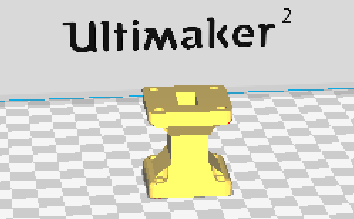
\includegraphics[scale=1.2]{Figs//waveguide_design.PNG}
  \caption[The waveguide design in Cura]{\footnotesize The waveguide design in Cura.}
  \label{Fig:waveguide}
\end{figure}
\\
More importantly, the filament samples containing different proportions of pumice was investigated to check the limitation and the influence of pumice for 3D printing, including reliable printing speed, build platform adhesion, the extruding temperature and geometrical accuracy of prints. 

\section{Thesis Outline}

The remainder of this thesis is structured as follows:
\begin{itemize}
\item Chapter Two describes the literature review of 3D printing systems, materials and the well-down research of 3D printing in the space.
\end{itemize}
\begin{itemize}
\item In Chapter Three and Four, it is shown that the actual experiments on filament production of ABS and pumice. The principle we complied with and findings when working with extruder and controller would be mentioned in detail.
\end{itemize}

\begin{itemize}
\item The investigation of the printing properties of filament is presented in Chapter Five.
\end{itemize}

\begin{itemize}
\item  At last, Chapter Six contains the conclusion of this project.
\end{itemize}



\chapter{Literature Review}
\renewcommand{\baselinestretch}{\mystretch}
\label{chap:Litera}
%\setlength{\parindent}{0pt}

\section{3D printing system}

\PARstart{3}{D} printing is an old but energetic technology, which is also named as additive manufacturing(AM). This idea was put into practice for rapid prototyping at the end of the 1980s and the beginning of the 1990s  \cite{long20173d} . In recent years, its development has attracted extensive interest from people in different fields. 3D printing has become one of the most popular manufacturing techniques in the industry. It has influenced mechanical manufacturing, architecture and medical fields. \\
\\
In the last decade, the cost of 3D printing system has dropped dramatically. In fact, 3D printing is getting into common usages and imaginations, which even be facilitated in families and companies. People could print their own designs with a 3D printer. More and more 3D printers have been designed  with a low price and the simple operations. A variety of raw materials have been investigated in 3D printing field. It is no surprise that 3D printing has been targeted as a reliable production technique. There are three groups of systems for additive manufacturing, which are recognised as liquid-based systems, solid-based systems and powder-based systems. The classification of 3D printing is organised in Figure \ref{Fig:classification}. In below, the most popular technique from each group will be introduced. 

\begin{figure}[htbp]
  \centering
  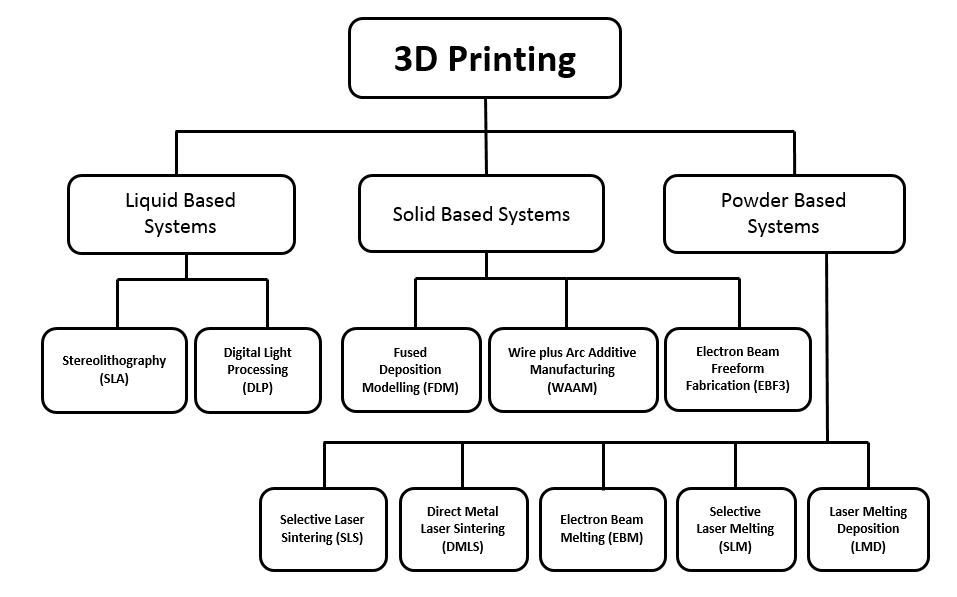
\includegraphics[scale=0.5]{Figs//3D_print_classification.PNG}
  \caption[The classification of 3D printing techniques]{\footnotesize The classification of 3D printing techniques.}
  \label{Fig:classification}
\end{figure}


\subsection{Stereolithography apparatus}

In history, Stereolithography apparatus (SLA) is the earliest 3D printing technology which was invented by Charles (Chuck) Hull in 1986. From then, SLA opened the door to commercialize the Rapid Prototyping (RP) system \cite{zhou2000parametric}. Stereolithography is based on laser technology and it belongs to the liquid-based system group. In the SLA 3D printing system as Figure \ref{Fig:SLA} presents, a UV laser scans the surface of the liquid resin then solidifies the layer selectively. The liquid material is contained in the tank. The platform would be moved down after one layer is scanned. A new layer of liquid resin will be hardened. The repetition of layer solidification could obtain an entire 3D object. Also,  a computer is embedded in the machine which could control the platform and the laser by reading a STL file. \\
\\
Stereolithography paves a way to create a considerably accurate 3D build with short time and respectively low cost. Therefore, SLA has gained wide acceptance in different fields, such as jewellery models \cite{leong1998abrasive} , replicas of heart for simulation of surgical operation \cite{shiraishi2014development}, etc.\\
\\
In terms of the raw materials for SLA, resin-based photopolymers are the basic idea. These liquid materials could react by solidifying when they are cured by a high-powered laser or light source. In practice, the energy from the laser is significant in SLA printing and it is affected by several elements, such as the scan speed, the cured time, the light and the material \cite{chia2015recent}. The limitation of available photopolymers becomes the main weakness of this technology \cite{wang2016stereolithographic}. However, there is a definite possibility that a wide variety materials are combined with photopolymers as the candidates for SLA technique, including short fibre \cite{yunus2017short}, ZrO2-reinforced Al2O3 components \cite{licciulli2005laser} and epoxy, diethylene triamine and silica powder \cite{scarparo1996mechanisms}. 

\begin{figure}[t]
  \centering
  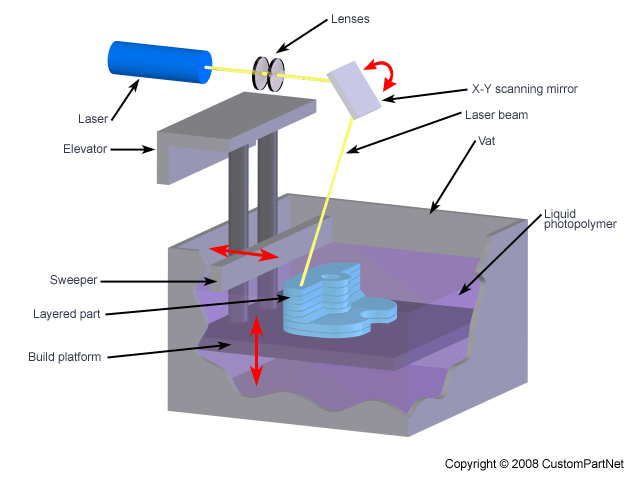
\includegraphics[scale=0.5]{Figs//SLA_PROCESS.png}
  \caption[SLA process]{\footnotesize SLA process.}
  \label{Fig:SLA}
\end{figure}

\subsection{Fused deposition modelling}

Fused Deposition Modelling (FDM) rapid prototyping system was firstly built by Scott Crump in 1988 \cite{hashmi2014comprehensive}, which is also known as Fused Filament Modelling (FFM). It is a considerably popular and low-cost technology for functional manufacturing. FDM system relies on filament extrusion \cite{carneiro2015fused}. In general, FDM system controls the nozzle head to produce all prints and the feature size of the production is limited by the die size in nozzle correspondingly. The FDM system in Figure \ref{Fig:FDM} heats and melts thermoplastic material by a nozzle head. And the concept of selective deposition is also applied \cite{dul2016fused}. The filament is fed by the motor and it is molten through the heater inside. The liquefier moves through the nozzle die and solidifies to the thin filament \cite{singh2014process}. The nozzle head moves horizontally and deposits material according to the design for current layer. The build plate moves down vertically when the printer finished one layer. After fabrication of each layer, the 3D model is complete without any hardening \cite{jin2015quantitative}.\\
\\
In this technique, there are lots of elements or parameters could influence the quality of products such as surface roughness. In terms of the properties of the material, the extruding temperature is decided by their glass transition temperature. The humidity, density and adhesion property of the material also cannot be neglected \cite{chohan2016mathematical}\cite{costa2017estimation}. As for other settings in the machine, the orientation, layer thickness, air gap, raster angle and width should be taken into consideration \cite{rao2016optimization}. Meanwhile, there are several build parameters which affect production accuracy and manufacture efficiency as well \cite{griffiths2016effect}\cite{boschetto2016design}.
 
\begin{figure}[htbp]
  \centering
  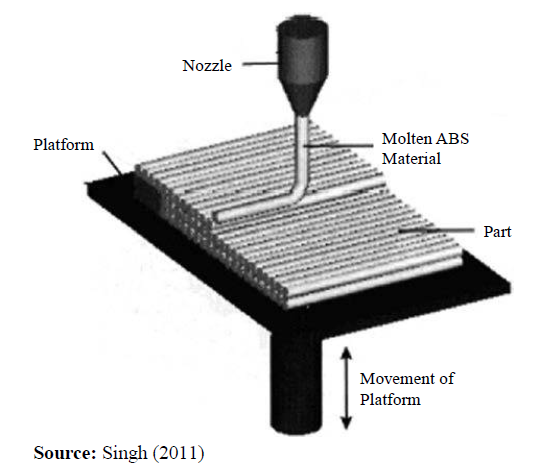
\includegraphics[scale=0.6]{Figs//FDM_process.PNG}
  \caption[FDM process]{\footnotesize FDM process.}
  \label{Fig:FDM}
\end{figure}

\subsection{Selective laser sintering}

Selective laser sintering uses layer printing to build a 3D model\cite{hashmi2014comprehensive}. It selectively fuses small particles of plastic, metal, ceramic or glass powders by a high power laser beam\cite{jiang2013study}. As can be seen in Figure \ref{Fig:SLS}, the materials for this process are powders which is placed in the container initially and spread on the building platform later. The building platform is lowered down every single layer finishes scanning by the laser according to its geometrical design\cite{shahzad2013additive}\cite{shahzad2014additive}. This procedure is repeated until the print is complete\cite{ganeriwala2014multiphysics}. \\
\\
This technique is without material moulding. Parts possess high mechanical properties\cite{zhu2015investigation}. This process is quite fast for printing functional, durable parts. It enables complex parts with interior components and without rapping the material inside and altering the surface from support removal. What’s more, there are vast variety of materials which could be applied for this technique, such as polypropylene (PP) powder \cite{zhu2015investigation}, PA12 and PEKK \cite{peyre2015experimental}, nanoparticle agglomeration\cite{yuksel2016modeling}. In fact, SLS regards Nylon based materials as the candidate materials. The weakness of this technique is the surface porosity of SLS printed parts. 

\begin{figure}[htbp]
  \centering
  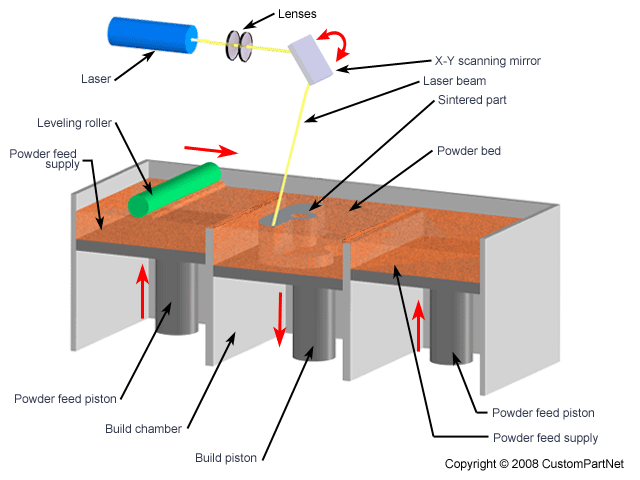
\includegraphics[scale=0.5]{Figs//SLS_process.png}
  \caption[SLS process]{\footnotesize SLS process.}
  \label{Fig:SLS}
\end{figure}

\section{3D printing materials}

The remarkable development of 3D printing technology provides insights into usage of various plastic polymers. The usage of virgin material is no more common since its high cost and time-consuming. Otherwise, people utilise the basic 3D printing materials as the base to combine with metal oxides, short fibres and other polymers as a new material to obtain some special properties \cite{torrado2015characterizing}. Since there are lots of durable and compatible plastic, it could be renewed and reused after adding the virgin material. \\
 \\
In fact, there are several popular thermoplastics for industrial manufacturing as well as personal work since they are low-cost and compatible. According to their different physical and chemical properties, they are applied for additive manufacturing with different techniques or settings. In figure \ref{Fig:material-per-stampanti}, it is clear that the products printed with PLA, ABS and Nylon are distinct. Furthermore, the details of these three materials would be explained below.
\\
\begin{figure}[htbp]
  \centering
  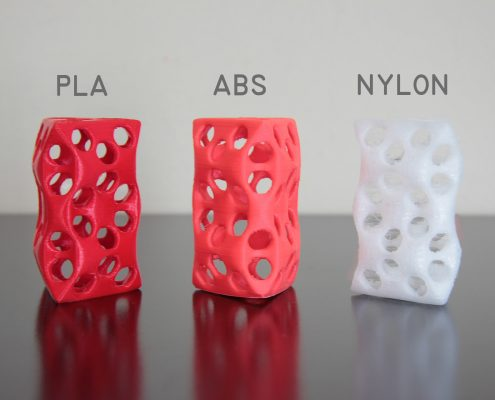
\includegraphics[scale=0.5]{Figs//materiali-per-stampanti-3D.jpg}
  \caption[3D prints made of different materials]{\footnotesize 3D prints made of different materials.}
  \label{Fig:material-per-stampanti}
\end{figure}

\subsection{Acrylonitrile butadiene styrene}

Acrylonitrile butadiene styrene (ABS) is a kind of thermoplastics polymer which plays a significant role in FDM rapid prototyping system. As the name suggests, ABS is composed of polymerising styrene and acrylonitrile in the presence of polybutadiene. ABS has no real melting point and its glass transition temperature is about 105 $^{\circ}$C (221 $^{\circ}$F)\cite{rutkowski1986acrylonitrile}.  ABS could be recycled and it is environmentally friendly. It is usually utilised between 20 and 80 $^{\circ}$C (−4 and 176 $^{\circ}$F) since it remains a relatively stable at a low temperature.\\
\\
Based on its mechanical properties, its impact resistance and high tensile strength enable it to build durable products, like the famous Lego bricks and other outer bodies of office facilitates. Its electrical property paves a new way to produce light and cost-effective electrical components, which work well over a wide range of frequencies. It is not surprised that 3D printed electromagnetic structures such as antenna\cite{mirzaee2015developing} and insulator\cite{mehmood2017performance} are made by ABS materials. ABS has attracted lots of interest from people since they could DO-IT-YOURSELF (DIY) with ABS filament at home. It is easy to design or download models from the Internet and print them to get some lovely products as Figure \ref{Fig:ABS product} shows.

\begin{figure}[htbp]
  \centering
  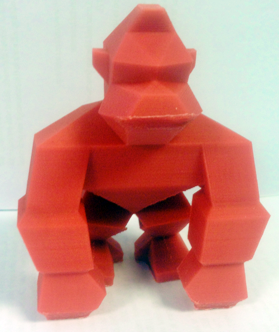
\includegraphics[scale=0.9]{Figs//ABS_product.png}
  \caption[3D-printed King Kong made of ABS]{\footnotesize 3D-printed King Kong made of ABS.}
  \label{Fig:ABS product}
\end{figure}

\subsection{Polylactic acid}

Polylactic acid (PLA) is similar to ABS for its renewable property. In particular, PLA belongs to bioplastic due to its biodegradable and bioactive properties. There are several types of PLA including PLLA (Poly-L-lactic Acid), PDLA (Poly-D-lactic Acid) and PDLLA (Poly-DL-lactic Acid) which are all derived from the renewable resource called lactic acid\cite{sodergaard2010industrial}. What should be concerned is the glass transition temperature of PLLA is between 60 and 65 $^{\circ}$C and its melting point is 157 - 170 $^{\circ}$C. It means PLA cannot be applied at a high temperature. In additive manufacturing, the typical injection moulding temperature of PLLA is about 178 - 240 $^{\circ}$C.\\
\\
More importantly, PLA is extremely robust in the normal application. Compared with ABS, PLA is a little bit less toxic and non-petroleum. And it is widely utilised in food packaging\cite{marra2017assessment} and medical implants\cite{bergstrom2016overview}. As a kind of dielectric material, PLA is also taken into use for antenna production\cite{mirzaee2016high}. PLA is also compatible and there are several PLA blends, such as Aluminum PLA as Figure \ref{Fig:PLA product} below .

\begin{figure}[htbp]
  \centering
 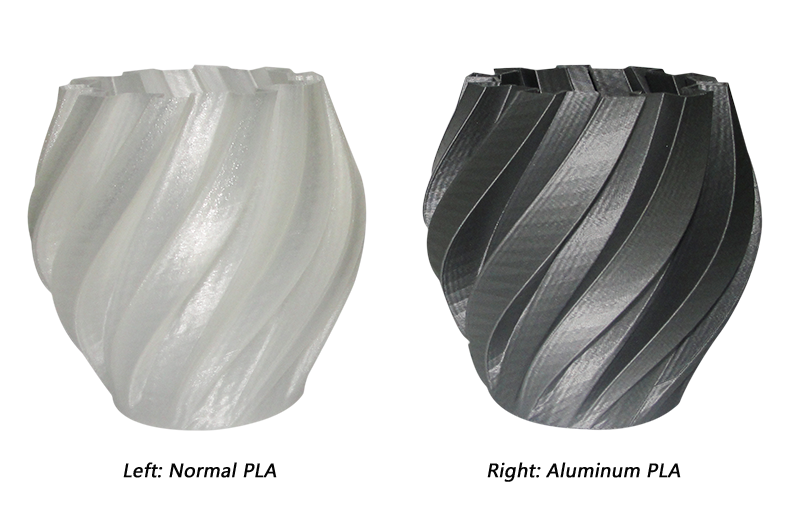
\includegraphics[scale=0.4]{Figs//aluminum-PLA_2.png}
  \caption[Pure PLA and Aluminum PLA products]{\footnotesize Pure PLA and Aluminum PLA products.}
  \label{Fig:PLA product}
\end{figure}


\subsection{Polyamide}

Nylon stands for a family of synthetic polymers. It was first invented by Dr. Wallace Hume Carothers as an ideal synthetic fibre in 1927 \cite{doi:10.1021/ed021p88}. With the development of Nylon production, it has become a kind of smooth thermoplastic material that could be fabricated into shapes, fibres or films. Pure Nylon has the critical problem about storage as it always absorbs moisture from the air and it is difficult to dry it. Therefore, people blend nylon with other fibres or polymers creatively to get an exceptionally durable Nylon blends.\\
\\
 In 3D printing, Nylon is a considerably attractive material for SLS technique \cite{shaw2016investigation}. In addition, there exists Nylon filament which is a candidate material for FDM system. Nylon filament is an incredibly durable, versatile and strong AM material. It is flexible with very high adhesion. Its low friction coefficient and high melting temperature are beneficial for FDM technique. In this case, application of Nylon varies from Artificial Muscles\cite{arjun2016design}, Nylon tube \cite{webb2006integration} to polyamide lens \cite{bunea2014investigation}.
 
\section{3D manufacture in space}

As it is mentioned before, there is an urgent requirement to apply 3D printing in space for long-term research. Actually, it has been verified that FDM technique is suitable and safe in the micro-gravity environment of the International Space Station\cite{fateriadditive}. Moreover, scientists also use 3D printing in aerospace by using a special Zero-Gravity 3D printer \cite{joshi20153d}. \\
\\
In fact, there are several groups researching on the In-situ resource utilisation for sustainable development of 3D printing in space \cite{kading2015utilizing}. In recent years, Lunar and Martian regolith in space are not mysterious for human beings anymore. Based on their multi-component ceramic property, there is no doubt to utilise them in the powder based system that is Selective Laser Melting (SLM) system \cite{goulas20163d}. However, it has been demonstrated that only lunar dust is a suitable material for this system while Martian dust is not \cite{goulas2017assessing}.  Additionally, there is a weakness of this technique with Lunar dust that the geometrical accuracy of the product should be improved \cite{fateriadditive}. And the vacuum environment is also a challenge for SLM technique.\\
\\ 
According to these studies, utilisation of Lunar and Martian regolith for FDM technique has emerged as an interesting topic. The combination of lunar/martian regolith and bio-derived polymers was successfully utilised for 3D printing \cite{jakus2017robust} as Figure \ref{Fig:lUNAR PRITNS} presents. Therefore, there is a strong possibility to produce other blends by mixing these two types of regolith with other printable polymers\cite{ray2010jsc}. 
 \\
 
\begin{figure}[htbp]
  \centering
  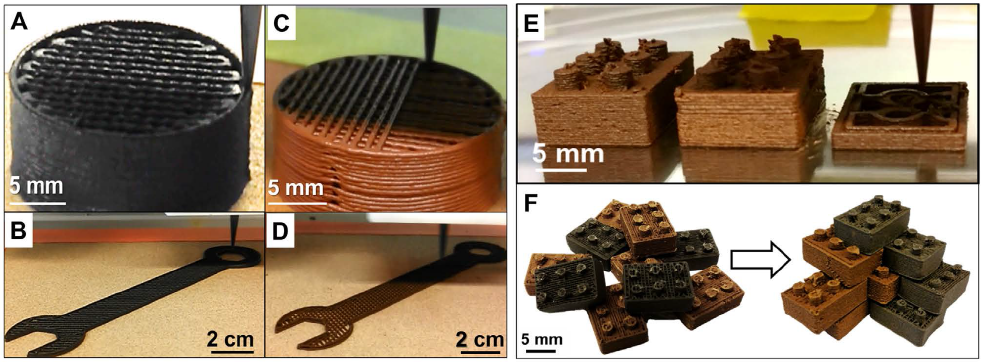
\includegraphics[scale=0.5]{Figs//LUNAR_dust_prints.PNG}
  \caption[3D-printed products made of Lunar/Mars dust]{\footnotesize 3D-printed products made of lunar dust(A,B), martian dust (C,D,E) and both (F) inks copyright @ 2017Robust. }
  \label{Fig:lUNAR PRITNS}
\end{figure}


\chapter{ABS Filament Production}
\renewcommand{\baselinestretch}{\mystretch}
\label{chap:ABS}
%\setlength{\parindent}{0pt}

\section{Methodology}
The aim of this project is producing printable filament with Lunar and Mars dust simulants. First of all, it is essential to test the printability of the basic material that is ABS pellets (INEOS Styrolution Group GmbH, Germany) and get suitable candidate filament for our 3D printer (Ultimaker 2 GO; Ultimaker B.V., Netherlands). The extruder called Noztek Pro in our experiment is produced by Noztek Company (England, UK), which offers fast extrusion of ABS pellets with tight tolerances. For the good quality of filament, the filament winder (Noztek, England, UK) worked with the extruder as Figure \ref{Fig:extruder and winder} shows.

\begin{figure}[htbp] % make the image in the middle of paragraph
	\centering
	\subfigure[]{
	\begin{minipage}[t]{0.4\textwidth}
			\centering
			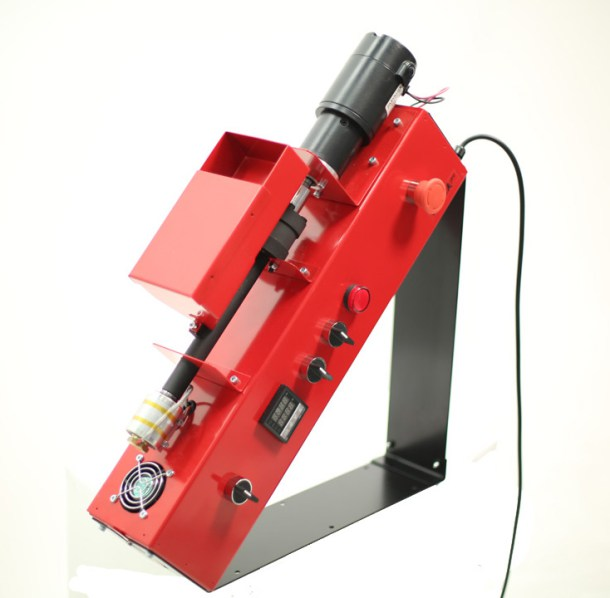
\includegraphics[height=6.1cm]{Figs3//noztek_pro.jpg}
		\end{minipage}
	}
	\subfigure[]{
		\begin{minipage}[t]{0.4\textwidth}
			\centering
			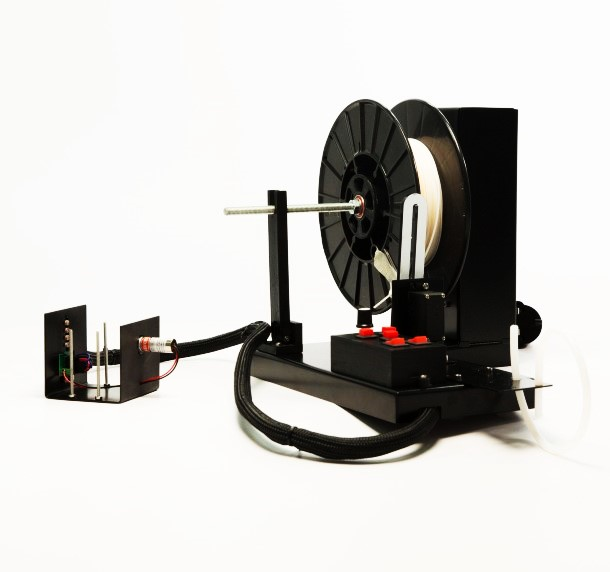
\includegraphics[height=6.1cm]{Figs3//winder1-crop.jpg}
		\end{minipage}
	}
  \caption[The machines for filament manufacuring]{\footnotesize (a) The extruder,(b)the filament winder. Copyright@ Noztek Co. }
  \label{Fig:extruder and winder}
\end{figure}

\subsection{ABS pellets}
As mentioned in Chapter Two, ABS was chosen as the base material due to its compatible property and the reasonable price. The mechanical properties like impact resistance and roughness\cite{swetham2017critical} of ABS also were taken into consideration.
In the view of the ABS pellets in Figure \ref{Fig:ABS pellets}, the colour is white and the size is fairly uniform. It should be noted that the storage of ABS pellets is significant as ABS pellets could absorb moisture from the air in general. As the ABS pellets were purchased in bulk, the solution was to separate the big bulk of pellets into small bags and keep them in a desiccator with desiccants before extrusion. Approximately, each kilogram of ABS pellets could produce 30 meters filament with 3mm diameter. Based on this approximation, 25kg ABS pellets were prepared for the total study.

\begin{figure}[t]
  \centering
  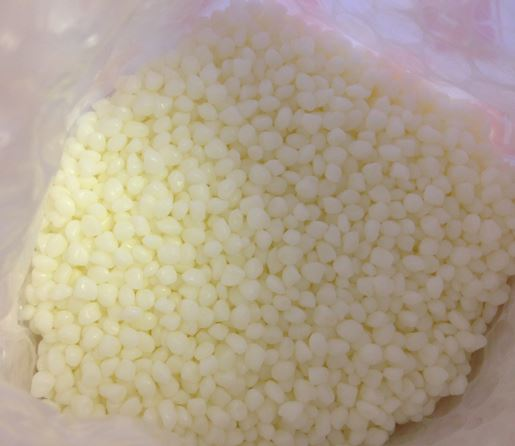
\includegraphics[scale=0.5]{Figs3//ABS_pellets.JPG}
  \caption[ABS pellets]{\footnotesize ABS pellets.}
  \label{Fig:ABS pellets}
\end{figure}

\subsection{Installation of Extruder and Winder}
In the factory, there are five steps for filament production, including extrusion with the extruder, cooling by a water tank, pulling with pull roller, cutting or removal by controlled winder and drying. As there was no oven or other available drying facilities, only the extruder and filament winder with a sensor were facilitated for filament manufacturing in this project. The composition of the extruder is described in Figure \ref{Fig:extruderexp}.\\
\\
In FDM 3D printing, it is necessary to note that the computer controls the printing process by calculating the extruded material's volume, which relies on the extrusion speed, the size of the die in nozzle head and the diameter of the filament. To be specific, the 3D printer controls the filament feeder to push a certain length of filament out of the nozzle by supposing its diameter is consistent. In this way, the unstable filament will cause the volume of extruded plastic changeable since the computer cannot identify the diameter variation. Therefore, the printing is continued with a setting of filament diameter and the printer expects a certain volume of material to come out. This trouble called inconsistent extrusion results from the poor diameter tolerance of filament.\\
\\
In order to avoid this bad printing, the ideal diameter of the filament is 2.85mm for Ultimaker 2 printer. Unfortunately, there are only two sizes of dies we can choose for extrusion nozzle, which are designed for the 1.75mm and 3mm filament production respectively. Consideration of ABS expansion at high temperature, the 1.75mm die was installed.  \\
\\
The reason why we facilitate filament winder is that it could improve the filament tolerances and collect all extruded filament neatly onto the spool. The filament winder was installed on a more robust chassis to offer the smooth and stable winding of 1Kg of the filament. It also connects a sensor and programmable laser module which calculates the extrusion speed of filament by monitoring the height of the filament, in turn changing the speed of the spool motor to give tangle free winding.\\
\\
The guide work of filament winding is similar to a fishing reel leveller. It is related to the spool motor's work record. The guiding part is programmed to rotate about 1 degree after each circle rotation of the spool. In fact, the extrusion product is winded on a standard wound spool which can be used directly to the 3D printer. Since there were not enough available spool for our samples, we re-winded the filament from the installed spool every time we finished extrusion.\\
\\
The entire system could be seen in Figure \ref{Fig:system}. The extruder was located on the desk in order to let filament drop down naturally while the winder was put on a lower place with the sensor in the middle of them. The vertical drop and horizontal distance between each machine would be adjusted during the experiment.

\begin{figure}[htbp]
  \centering
  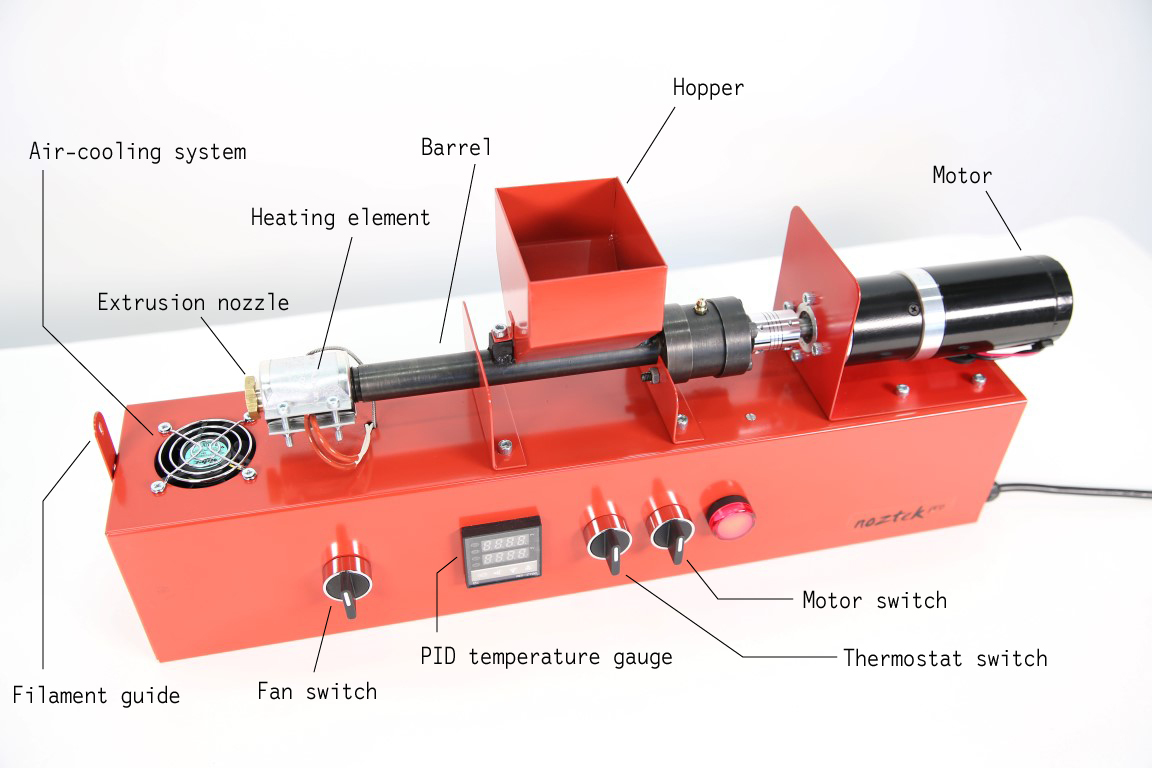
\includegraphics[scale=0.3]{Figs3//Noztekexplained.jpg}
  \caption[Details of the extruder]{\footnotesize Details of the extruder.}
  \label{Fig:extruderexp}
\end{figure}
\begin{figure}[htbp]
  \centering
  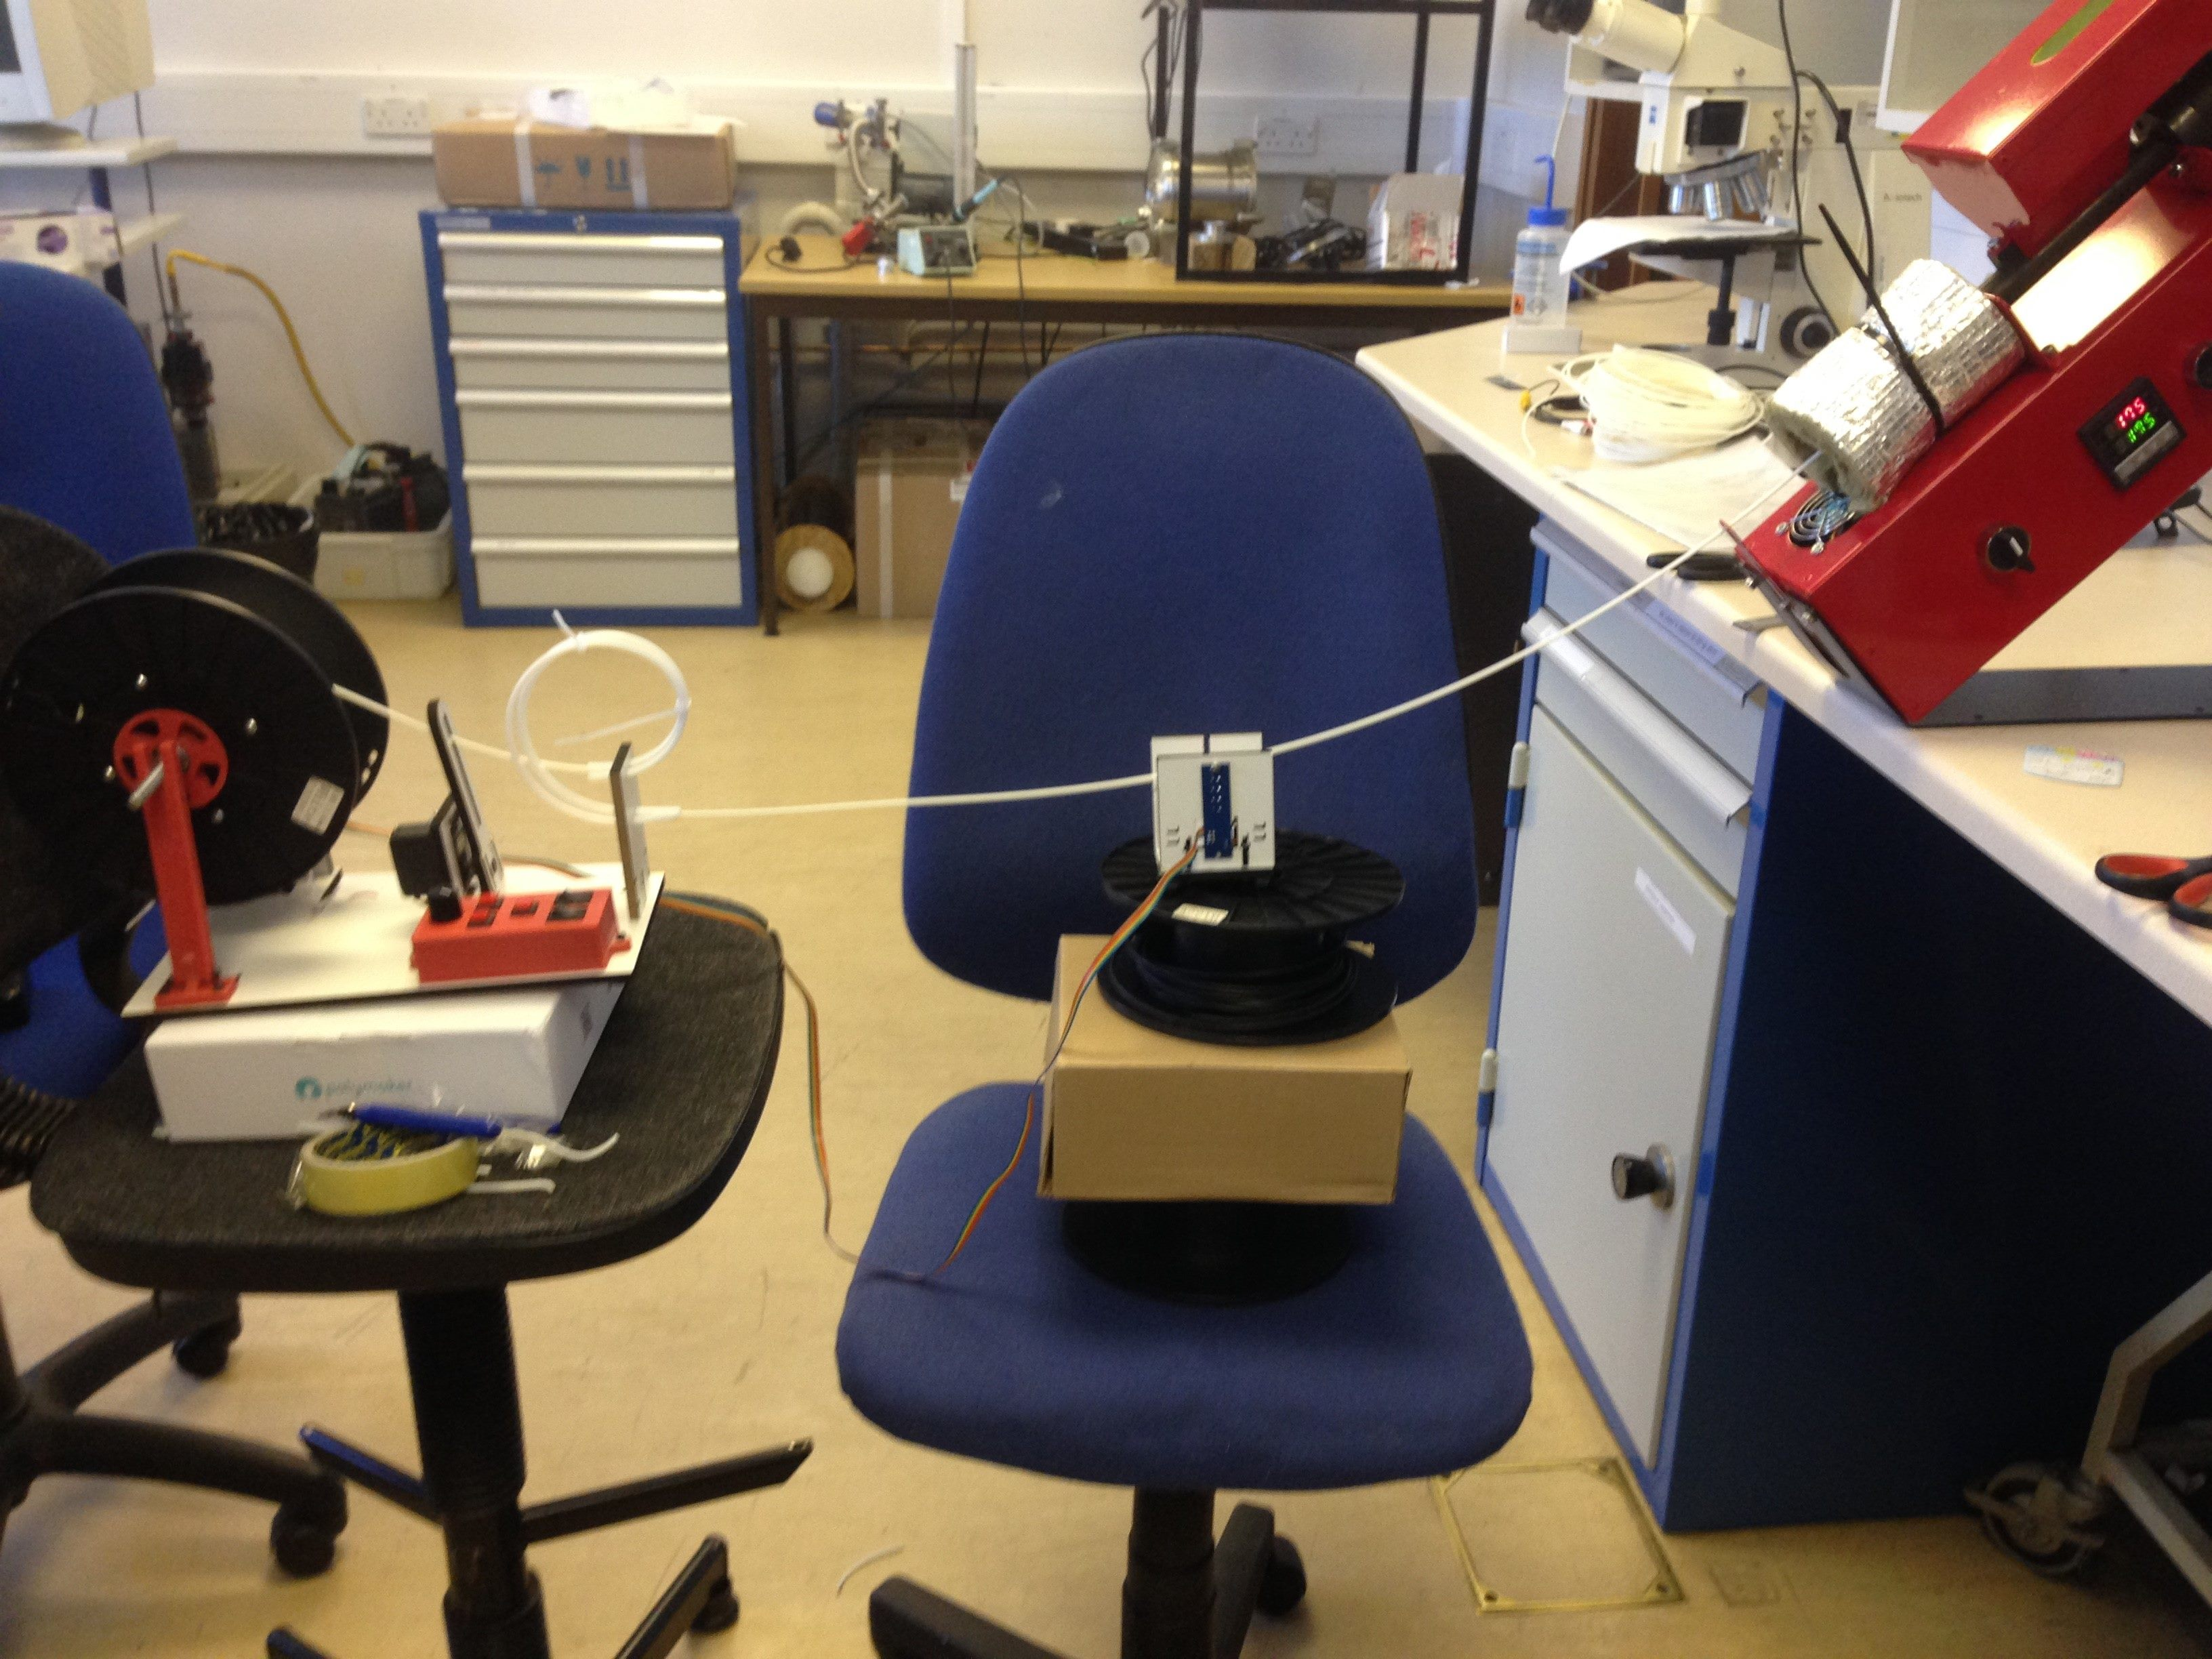
\includegraphics[scale=0.1]{Figs3//system.jpg}
  \caption[The extrusion system]{\footnotesize The extrusion system.}
  \label{Fig:system}
\end{figure}

\section{Experiment}
\subsection{Consideration of Process Parameters}
There are several settings in process we should consider in the experiment:
\begin{itemize}
\item Extruding temperature
\end{itemize}
In principle, if the extrusion speed is too slow, the temperature needs to be increased. If the filament stretches out too much or curls up right as it comes out of the nozzle, the temperature needs to be decreased. Firstly, we chose 190 $^{\circ}$C as a test according to the data sheet of the ABS pellets.
\begin{itemize}
\item Position of the sensor and winder
\end{itemize}
The location of sensor and winder depends on the whether it can control the winder’s speed appropriately which makes the filament 10-30 cm below the nozzle to avoid increased sketching. Meanwhile, it is required that the filament does not touch anything until it is cool down.
\begin{itemize}
\item Controller of the winder
\end{itemize}
The design of the filament winder offers two methods to control the winding speed:
\\
By sensor: The sensor could control the motor which is connected to the spool.It is more flexible but it needs the fine setting of the calibration and fine tuning of the position of the sensor. Since the limited sensitivity of the sensor, it might make the winder speed up sharply which causes that the filament is not uniform enough.
\\
Manually control: There is a button on the platform of the winder to control its rotating speed. This method needs more attention paid on extruder and filament. And it seems difficult to find a speed of winder which exactly corresponds to the speed of filament extruding so the speed is required to be adjusted again and again.
\begin{itemize}
\item Utilisation of fans
\end{itemize}
Since there is no water bath installation in our system, the cooling of filament depends on the air temperature and the use of fans. The air temperature in our laboratory was controlled at 24 $^{\circ}$C all the time. There are two fans we can choose. One was the small fan installed in the extruder and the other was a big fan.
Turning on the both fan would cause that the extruding temperature is not static and the diameter of the filament shrinks. But the filament could cool down faster.

\subsection{Investigation of Process Parameters}
Firstly, we compared the manual control and sensor control filament extrusion. The differences between them are not very clear. After fine calibration, the sensor could make life easier. We used sensor to control the rotation of spool in the following experiment.\\
\\
The second parameter that paid attention to was the use of fans. There was no cooling installation in our system. Only the air-conditioner in the laboratory could make progress on rapidly cooling of ABS filament. Since we want to obtain 2.85mm diameter of the filament with a 1.75mm die, it is better to cool the filament rapidly when it expands through the nozzle head.
The fan of extruder was exactly installed at the right place that the filament was very hot. Another facility that made sense was the big fan which can enable the filament to cool down entirely before it was collect by the spool.\\
\\
In the view of the idea above, we did several tests with the same position of sensor and filament winder. The diameter of the extruded filament was measured by a digital calliper at the different place of the filament. The results and corresponded parameters are described in Table \ref{tab:fan}. During the experiment, the big fan was set to the lowest power and located 50cm far from the filament to ensure the filament does not swing by the wind. The diameter of the filament is continuously variable so the measurement result is described as a range. Setting the same extruding temperature, the utilisation of any fans was detrimental to the stability of diameter. In detail, turning on the extruder fan made the filament shrinks a lot while the big fan increases the uncertainty of the diameter (changeable in a bigger range). In order to achieve a more consistent diameter and minimize the difference, it is reasonable to turn off all the fans.\\
\\
There is an interesting parameter in Table \ref{tab:fan} we should analyse as well. The extruding temperature has a strong effect on filament diameter. It was indicated that the higher extruding temperature offers a bigger filament size to some degree from 175$^{\circ}$C to 200$^{\circ}$C. This conclusion should be verified definitely by more professional work. Another principle that the higher temperature offers the faster extrusion was totally true at this stage. The most important thing was to decide an extruding temperature offering the stability and suitable size of the filament. 
\begin{table}[t]
\centering
\caption{Usages of fans for filament production}
\begin{tabular}{c c c c}
\hline
\textbf{Temperature} & \textbf{Extruder Fan} & \textbf{Big Fan} & \textbf{Filament Diameter}\\
\hline
170$^{\circ}$C & off & off & 2.65-2.75mm \\
170$^{\circ}$C & on & off & 2.60-2.72mm\\
170$^{\circ}$C & on & on & 2.41-2.61mm  \\
175$^{\circ}$C & off & off & 2.72-2.98mm \\
175$^{\circ}$C & off & on & 2.67-3.17mm\\
185$^{\circ}$C & off & off & 2.71-2.90mm \\
185$^{\circ}$C & off & on & 2.32-2.61mm\\
185$^{\circ}$C & on & off & 2.34-2.54mm  \\
190$^{\circ}$C & off & off & 2.67-2.87mm \\
190$^{\circ}$C & off & on & 2.43-2.88mm \\
190$^{\circ}$C & on & on &  2.35-2.62mm\\
200$^{\circ}$C & on & off & 2.32-2.52mm \\
200$^{\circ}$C & off & on & 2.59-2.89mm \\
200$^{\circ}$C & on & on & 2.18-2.61mm \\
\hline
\end{tabular}
\label{tab:fan}
\end{table}\\
It is time to judge the best installed position of sensor and filament winder.  
\begin{enumerate}
\item Vertical drop\\
The vertical distance is between nozzle head of extruder and the platform of filament winder. And the sensor is located in the lowest place of the extruding filament between the winder and extruder. It is general to keep winder and filament on the same horizontal platform which results in a parabola shape of extruded filament between them. It seems to require a long horizontal distance for filament flowing. In the aspect of the shrink of the filament in this way, we chose a small but non-negligible vertical drop to fabricate big size filament.
\item Horizontal distance\\
The horizontal distance means the distance between nozzle head of extruder and the guiding pipe of winder system. The setting of this parameter is related to the vertical drop, the goal is to control the stretch strength of winder to manufacture the filament with a suitable size.
\end{enumerate}
\begin{table}[t]
\centering
\caption{Extrusion parameters for filament production}
\begin{tabular}{c c c c}
\hline
\textbf{Temperature} & \textbf{Vertical Drop} & \textbf{Horizontal Distance} & \textbf{Filament Diameter}\\
\hline
170$^{\circ}$C & 30cm & 60cm & 2.65-2.75mm \\
175$^{\circ}$C & 30cm & 60cm & 2.72-2.98mm \\
175$^{\circ}$C & 25cm & 60cm & 2.87-3.03mm \\
180$^{\circ}$C & 30cm & 60cm & 2.52-2.80mm \\
180$^{\circ}$C & 30cm & 45cm & 2.95-3.04mm \\
185$^{\circ}$C & 10cm & 80cm & 2.71-2.90mm \\
190$^{\circ}$C & 10cm & 60cm & 2.67-2.87mm \\
190$^{\circ}$C & 20cm & 40cm & 2.78-3.00mm \\
195$^{\circ}$C & 20cm & 45cm & 2.72-2.89mm \\
200$^{\circ}$C & 10cm & 60cm & 2.59-2.89mm \\
200$^{\circ}$C & 20cm & 60cm & 2.64-2.84mm \\
210$^{\circ}$C & 30cm & 60cm & 2.50-2.70mm \\
220$^{\circ}$C & 20cm & 60cm & 2.45-2.65mm \\
\hline
\end{tabular}
\label{tab:tems}
\end{table}
In Table \ref{tab:tems}, there are three parameters that the size of filament contributes to. The vertical drop is related to the stability and the size of the filament. The big vertical drop increases the consistency of filament while it decreases its size. The relation between horizontal distance and diameter is obviously proportional. By analysis of these results, it is suitable to choose 20cm vertical drop and 60cm horizontal distance.  As for temperature, the range from 185$^{\circ}$C to 195$^{\circ}$C could be taken into practice.\\
\\
During the experiment, the colour of filament also attracted my attention. As can be seen in Figure \ref{Fig:filament}, the colour of filament is not uniform sometimes. Some part of it is off-white while other is white. The reason is complicated since the fabricated filament could be different even with the same settings. Our extruder is not professional and stable. But there is a need to keep the machines and ABS pellets under the good condition to improve the quality of production. 

\begin{figure}[t] % make the image in the middle of paragraph
	\centering
	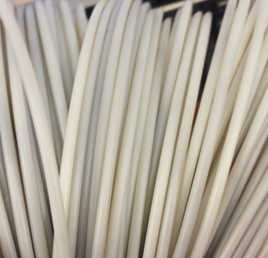
\includegraphics[scale=1]{Figs3//filament_colour.png}
  \caption[Pure ABS filament]{\footnotesize Pure ABS filament.}
  \label{Fig:filament}
\end{figure}

\section{Analysis}

According to all these results above, the optimization of all parameters could be found. It is concluded that there is a high probability to manufacture 2.85mm filament with 195$^{\circ}$C extruding temperature, 20cm vertical drop and 60cm horizontal distance. The best result with these settings is the filament at 2.85 $\pm$ 0.07mm. The diameter error is controlled within 2.5\%.\\ 
\\
It can not be avoided that the diameter of the filament is changeable because the extruding speed and filament wind speed are not stable. The extruder we used is not professional and the extruding system is simplified which may cause some weakness. Actually, the filament we bought does not have a specific diameter (e.g. 3.00 $\pm$ 0.05mm). This diameter tolerance (i.e. 0.05 mm) the gold standard across the industry. In this case, the filament we produced seems to been printable in Ultimaker 2 printer in the aspect of its diameter.\\
\\
As for the colour of filament, it does not make a big difference to its printing properties. Since the screw in the extruder is not long enough, the extrusion process is simplified. There is an uncertainty of the production because of the insufficient extruding.The tip is keeping the nozzle at the extruding temperature at least 20 minutes before the extrusion starts. And it is necessary to check the connection of every part and clean the hopper.\\
\\
It is also significant to storage our filament in an air tight container in order to print high-quality products\cite{abs}. The tricky thing with most thermoplastics is the moisture absorption, which results in small water bubbles in the filament. It will bring pops when extruding it in 3D printer. The extruding temperature is usually higher than the boiling point of water so that the water explodes violently. Obviously,  the quality of our 3D prints dramatically destroys since the material is spewed out randomly, instead of being correctly laid down. Also, it could cause spluttering and problems with adhesion on the base layer of the prints. There is a basic strategy to keep your 3D printing filament and avoid the accumulation of water from the atmosphere. It is very effective to store the filament in an air tight desiccator with a small silica gel desiccant pouch.\\

\chapter{Manufacturing with ABS and Pumice}
\renewcommand{\baselinestretch}{\mystretch}
\label{chap:Pumice}
%\setlength{\parindent}{0pt}

\section{Methodology}
\subsection{Pumice powder}
In this project, the central issue is to demonstrate that the Martian and Lunar Regolith could be utilised for FDM technique as a raw material. As revealed by Figure \ref{Fig:mars and pumice}(a), there are some particles with the diameter large than 0.1mm among martian regolith. Similarly, the particles of Lunar regolith in Figure \ref{Fig:lunar} are also not very uniform. In order to produce a printable filament for Ultimaker 2, it is required to sieve these kinds of regolith to remain the small particles of which the diameter is less than 100$\mu$m. In fact, the basic pumice powder (599907, Pumice Powder 6/0, very fine, Kremer Pigments) in  Figure \ref{Fig:mars and pumice}(b) has the size of 0 - 90$\mu$m which is exactly suitable. Pumice is a type of volcanic rock which makes up of highly vesicular rough textured volcanic glass. Based on the SEM pictures, this kind of pumice powder could be regarded as the substitution of the Lunar and Mars dust in the experiment.  
\begin{figure}[htbp] % make the image in the middle of paragraph
	\centering
	\subfigure[]{
    \begin{minipage}[t]{0.47\textwidth}
			\centering
			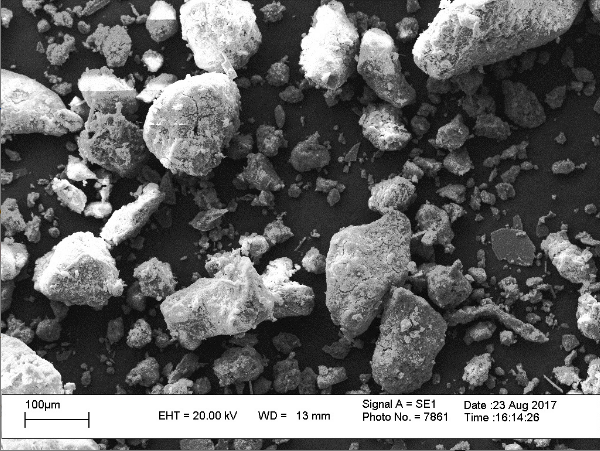
\includegraphics[height=5.5cm]{Figs4//mars_regolith.PNG}
		\end{minipage}
	}
	\subfigure[]{
		\begin{minipage}[t]{0.47\textwidth}
			\centering
			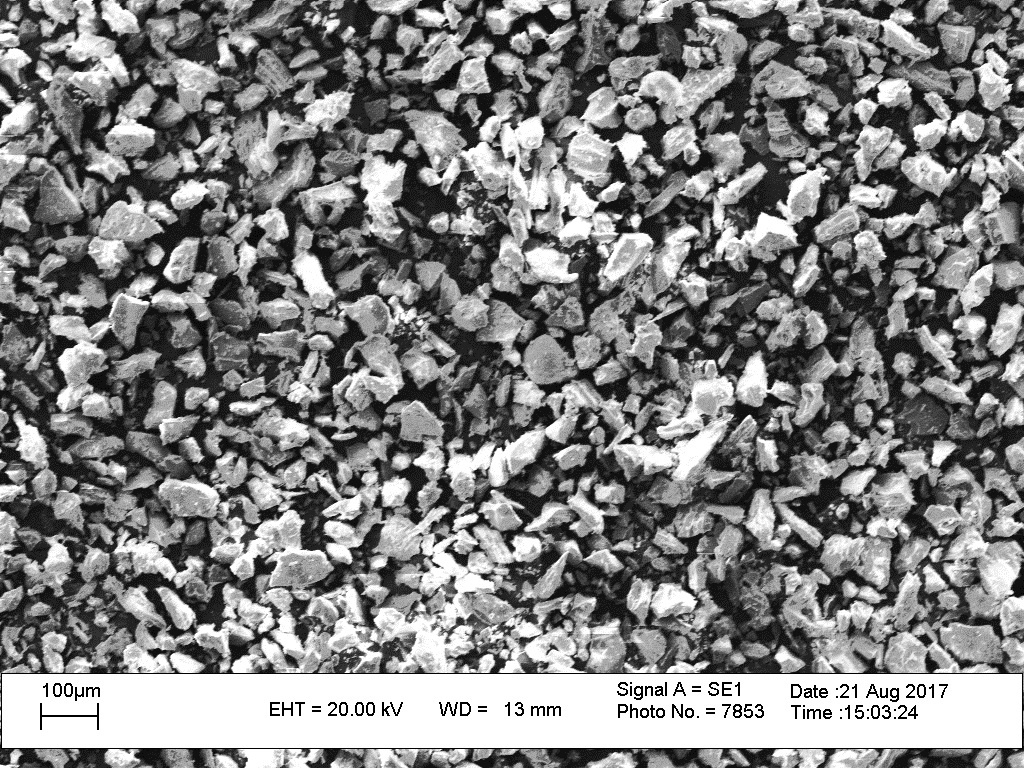
\includegraphics[height=5.5cm]{Figs4//pumice.jpg}
		\end{minipage}
	}
  \caption[SEM pictures of martian regolith and pumice powder]{\footnotesize SEM pictures of(a)martian regolith,(b) pumice powder.}
  \label{Fig:mars and pumice}
\end{figure}
\begin{figure}[htbp] % make the image in the middle of paragraph
	\centering
	\subfigure[]{
    \begin{minipage}[t]{0.47\textwidth}
			\centering
			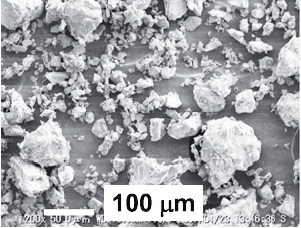
\includegraphics[height=5.5cm]{Figs4//fsd.PNG}
		\end{minipage}
	}
	\subfigure[]{
		\begin{minipage}[t]{0.47\textwidth}
			\centering
			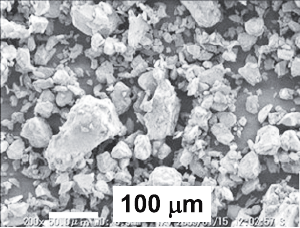
\includegraphics[height=5.5cm]{Figs4//JSC.PNG}
		\end{minipage}
	}

  \caption[SEM pictures of lunar regolith]{\footnotesize Lunar regolith simulants (a)FJS-1 ,(b)JSC-1. @copyright 2014 American Society of Civil Engineers.}
  \label{Fig:lunar}
\end{figure}
\subsection{Mixture of ABS and pumice}
Since the size and density of ABS pellets are very different from the pumice powder, it is not reasonable to directly pour them into the hopper of the extruder for the uniform filament. Ideally, powdering the ABS pellets into the same size of pumice powder could give the very uniform production. The methods to grind ABS pellets are very limited with the available facilities in our lab. And it is impossible to produce a ABS powder as fine as the pumice according to the elastic property of ABS. It is tricky that ABS material would be softened or even melted by the high power machine. The first method is to collect the small pieces of ABS by push 3mm ABS filament into a rotary tool/milling machine cutter. Another idea is using a mill coffee grinder to powdered the ABS pellets.\\
\\ 
Based on the powdered ABS and pumice, it is possible to produce the filament with different proportion of pumice and compare the weakness and advantages of specific samples. As for 3D-printability, the best way before printing is to check the consistency and smoothness of filament. 

\section{Experiment}

\subsection{Mixture of ABS and pumice with a funnel}
Firstly, the simple idea is that dropping the specific amount of ABS pellets and pumice powder into the screw with a controlled speed. The mixing work is in the dual-screw. It is not reliable to pour ABS pellets and pumice powder directly to hopper as the small particles always drop to the bottom. Based on the user's handbook of Noztek Pro Extruder, the extruding process with uniform raw materials has a relatively stable speed that we can calculate. The method was pouring a certain quantity of ABS pellets in the hopper and recording how long it takes to extrude all materials. The extrusion speed of ABS pellets at 195$^{\circ}$C in average is 0.1497g/sec. The challenge is the control of pumice powder dropping speed in order to control the amount of pumice in the filament. In this way, a funnel was designed(Figure \ref{Fig:funnel}) for guiding pumice powder. The installation of the funnel is revealed as Figure \ref{Fig:funnel install}.\\
\begin{figure}[htbp] % make the image in the middle of paragraph
	\centering
	\subfigure[]{
    \begin{minipage}[t]{1\textwidth}
			\centering
			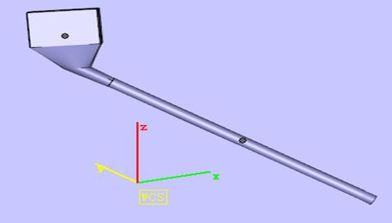
\includegraphics[width=9cm]{Figs5//funnel1.JPG}
		\end{minipage}
	}
	\subfigure[]{
		\begin{minipage}[t]{1\textwidth}
			\centering
			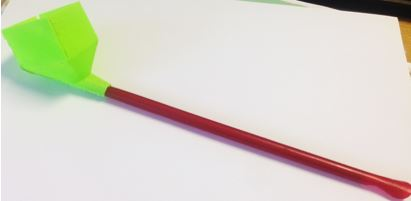
\includegraphics[width=9cm,height=5cm]{Figs5//funnel2.JPG}
		\end{minipage}
	} 
  \caption[The designed funnel]{\footnotesize (a)CAD profile of the funnel,(b)printed funnel with a screw.}
  \label{Fig:funnel}
\end{figure}
\\
After several adjusts, the pumice could drop into the hopper with a stable speed. However, the filament we got in this way is not uniform which can be seen in Figure \ref{Fig:fail}. This experiment failed since the ABS pellets covered the hole in the hopper to screw at first. The pumice powder and the ABS pellets cannot drop into the screw at the same time. The limitation of our equipment appeared in this test. Our extruder and its hopper were placed with 45 $^{\circ}$ angle to the horizontal plane. And one hopper extruder is not suitable for two different size particles extrusion together. It does not mean this method is not useful. There is a possibility that a dual-hopper extruder placed horizontally could produce homogeneous filament.

\begin{figure}[htbp] % make the image in the middle of paragraph
	\centering
	\subfigure[]{
    \begin{minipage}[t]{0.45\textwidth}
			\centering
			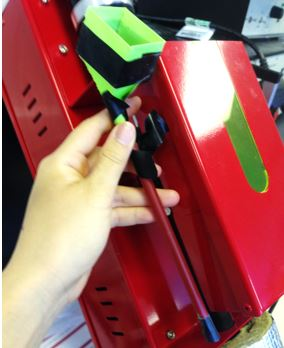
\includegraphics[height=8cm]{Figs5//funnel3.JPG}
		\end{minipage}
	}
	\subfigure[]{
		\begin{minipage}[t]{0.45\textwidth}
			\centering
			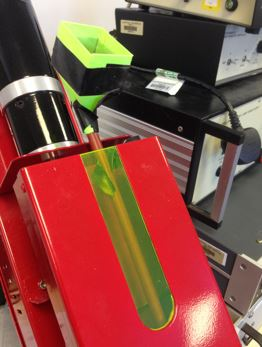
\includegraphics[height=8cm]{Figs5//funnel4.JPG}
		\end{minipage}
	} 
  \caption[The installation of the funnel]{\footnotesize The installation of the funnel.}
  \label{Fig:funnel install}
\end{figure}
\begin{figure}[htbp]
  \centering
  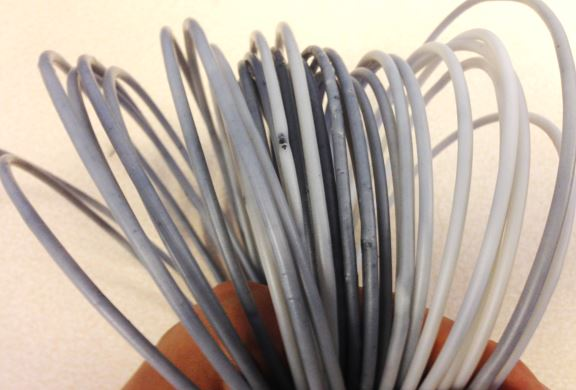
\includegraphics[scale=0.65]{Figs5//fail.JPG}
  \caption[The filament produced by the extruder and the funnel]{\footnotesize The filament produced by the extruder and the funnel.}
  \label{Fig:fail}
\end{figure}

\subsection{Mixture of ABS and pumice with a cutter}
The second method to powder ABS is using a manually-controlled cutter. The filament in Figure \ref{Fig:cutter} is with a diameter between 3.34-3.52 mm which is manufactured at 160 $^{\circ}$C. With the cutter in Figure \ref{Fig:cutter}(b), the ABS filament was powdered as \ref{Fig:cutter}(c).There are some big particles left. Compared with the size of pumice powder, this method risks the fabrication of uniform filament. After sieving these larger particles, we combined 38g powdered ABS with 2g (5 wt.$\%$) pumice powder, then used 195$^{\circ}$C as extruding temperature to obtain the filament which is very brittle and coarse\ref{Fig:filament}. Meanwhile, the powdered ABS easily absorbed moisture from the air which resulted in air bubbles in the filament.  

\begin{figure}[htbp] % make the image in the middle of paragraph
	\centering
	\subfigure[]{
    \begin{minipage}[t]{0.31\textwidth}
			\centering
			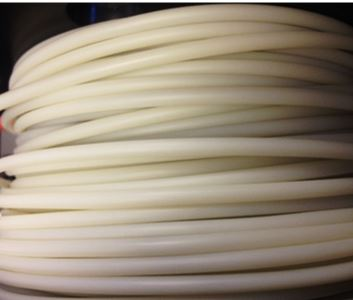
\includegraphics[height=4.2cm]{Figs4//big_filament.png}
		\end{minipage}
	}
	\subfigure[]{
		\begin{minipage}[t]{0.27\textwidth}
			\centering
			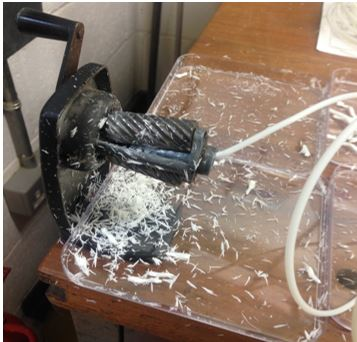
\includegraphics[height=4.2cm]{Figs4//cutter.jpg}
		\end{minipage}
	} 
 \subfigure[]{
		\begin{minipage}[t]{0.27\textwidth}
			\centering
			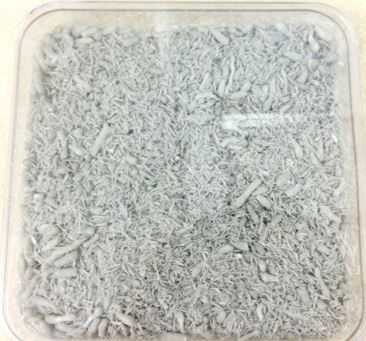
\includegraphics[height=4.2cm]{Figs4//cuttered_ABS.png}
		\end{minipage}
	}
  \caption[ABS pieces and the cutter]{\footnotesize (a)ABS filament,(b)the cutter,(c)powdered ABS .}
  \label{Fig:cutter}
\end{figure}

\begin{figure}[htbp] % make the image in the middle of paragraph
	\centering
	\subfigure[]{
    \begin{minipage}[t]{0.37\textwidth}
			\centering
			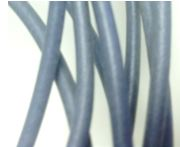
\includegraphics[height=4.5cm]{Figs4//filament.JPG}
		\end{minipage}
	}
	\subfigure[]{
		\begin{minipage}[t]{0.37\textwidth}
			\centering
			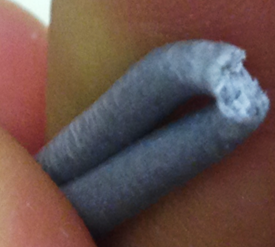
\includegraphics[height=4.5cm]{Figs4//filament_2.png}
		\end{minipage}
	}

  \caption[The quality of the filament]{\footnotesize  (a)coarse texture, (b)brittleness. }
  \label{Fig:filament}
\end{figure}

\subsection{Mixture of ABS and pumice with a coffee grinder}
Initially, the idea was use the coffee grinder (E5601BK, LLOYTRON, 150W) in Figure \ref{Fig:grinder}(a) to powder the ABS pellets. Unfortunately, it was really low-efficient work with this grinder and ABS pellets always be melted before it becomes small particles. Another problem that we cannot deal with is the moisture absorption during this process.\\
\\
After several tryings, the way to combine ABS and pumice could be worked for both the coffee grinder and the screw of extruder. The reason why we cannot pour the pumice powder and ABS pellets directly into the hopper of extruder is that the pumice powder always drops into the duality screw faster than ABS pellets. The main combination work of these two materials should be in the screw. In this view, the task of material preparation is to ensure the stable quantity of ABS and pumice drop into the screw/drill of the extruder at the same time. \\
\\
The pumice powder seems to be easily attached to slightly melted ABS pellets. The coffee grinder is used to implement this procedure creatively. The procedure as can be seen in Figure \ref{Fig:grinder}(b) and (c) is using the coffee grinder to mix ABS pellets and pumice together. This method is time efficient while the limitation obviously appeared is that the ABS cannot attach too much pumice. Moreover, the grinder will produce some ABS powder (Figure\ref{Fig:powder} after a long time grinding. In this way, there are several blends made by ABS pellets and 1 to 8 wt.$\%$ pumice are obtained. \\

\begin{figure}[htbp] % make the image in the middle of paragraph
	\centering
	\subfigure[]{
    \begin{minipage}[t]{0.25\textwidth}
			\centering
			
\includegraphics[height=5cm]{Figs4//grinder.jpg}
		\end{minipage}
	}
	\subfigure[]{
		\begin{minipage}[t]{0.27\textwidth}
			\centering
			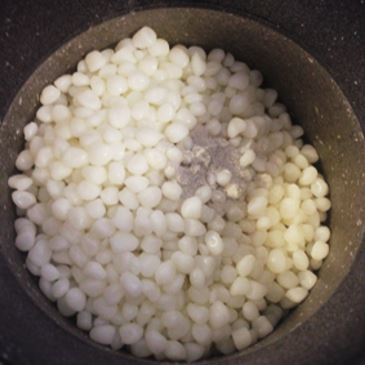
\includegraphics[height=5cm]{Figs4//abspumice1.JPG}
		\end{minipage}
	} 
 \subfigure[]{
		\begin{minipage}[t]{0.27\textwidth}
			\centering
			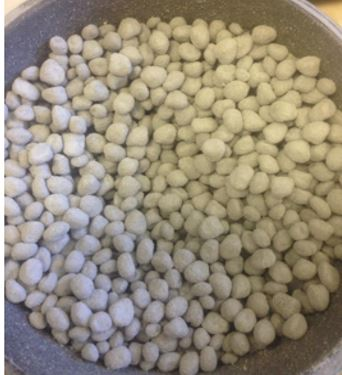
\includegraphics[height=5cm]{Figs4//abspumice2.JPG}
		\end{minipage}
	}
  \caption{Coffee grinder and the blends of ABS and pumice}{\footnotesize (a)Coffee grinder,(b)ABS and pumice,(c)blends of ABS and pumice.}
  \label{Fig:grinder}
\end{figure}

\begin{figure}[htbp] % make the image in the middle of paragraph
	\centering
	\subfigure[]{
    \begin{minipage}[t]{0.4\textwidth}
			\centering
			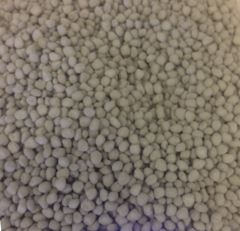
\includegraphics[height=6cm]{Figs4//abspumice3.JPG}
		\end{minipage}
	}
	\subfigure[]{
		\begin{minipage}[t]{0.4\textwidth}
			\centering
			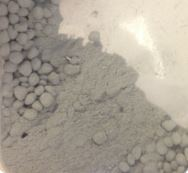
\includegraphics[height=6cm]{Figs4//powder.JPG}
		\end{minipage}
	} 

  \caption{ABS pellets and pumice powder}{\footnotesize  (a)ABS pellets with 8 wt.$\%$ pumice, (b)blends of ABS powder and pumice powder.}
  \label{Fig:powder}
\end{figure}

\subsection{Filament manufacturing}

In fact, it is significant to manufacture the 3D-printable filament with pumice powder at this stage. The key point for good printing is to make the diameter tolerance of the filament as small as possible.  Ideally, our filament should maintain an absolutely constant diameter as 2.85mm across the entire spool. However, due to small imperfections and our unprofessional extruder in the manufacturing process, there is always a tolerance of the filament diameter. In industry, the diameter tolerance could be as small as 0.05mm. It is obvious that the tolerance of our filament would be bigger than 0.05mm.\\
\\
Similar to the pure ABS filament production, the extrusion parameters could be adjusted according to the performance of products, especially the size of the filament. The performance of the filament and corresponded parameters are explained in Table \ref{tab:filament}. The mainly extruded materials are ABS pellets so that the extruding temperature could be the same as that of pure ABS. The most interesting thing is the filament shrinks when adding more than 6 wt.$\%$ pumice powder. The filament is fairly uniform as Figure \ref{Fig:FILAMENTS} shows with the exception of filament composited of ABS and 8 wt.$\%$ pumice. It is obvious that there are some blotches on the 8 wt.$\%$ pumice filament which suggests the distribution of pumice powder is not uniform. It exposes the limitation of this method that We can only make the good mixture with 7 wt.$\%$ pumice at most.\\

\begin{table}[htbp]
\centering
\caption{Extrusion parameters for filament production}
\begin{tabular}{c c c c}
\hline
\textbf{Temperature} & \textbf{Material} & \textbf{Horizontal Length} & \textbf{Filament Diameter}\\
\hline
195$^{\circ}$C & ABS with 1 wt.$\%$ pumice & 60cm & 2.78-2.98mm \\
195$^{\circ}$C & ABS with 2 wt.$\%$ pumice & 60cm & 2.85-3.05mm \\
195$^{\circ}$C & ABS with 3 wt.$\%$ pumice & 60cm & 2.83-3.03mm \\
195$^{\circ}$C & ABS with 4 wt.$\%$ pumice & 60cm & 2.84-3.02mm \\
195$^{\circ}$C & ABS with 5 wt.$\%$ pumice & 55cm & 2.84-2.97mm \\
195$^{\circ}$C & ABS with 6 wt.$\%$ pumice & 55cm & 2.80-2.92mm \\
195$^{\circ}$C & ABS with 7 wt.$\%$ pumice & 55cm & 2.77-2.88mm \\
195$^{\circ}$C & ABS with 8 wt.$\%$ pumice & 50cm & 2.65-2.75mm \\
\hline
\end{tabular}
\label{tab:filament}
\end{table}
\begin{figure}[htbp] % make the image in the middle of paragraph
	\centering
	\subfigure[]{
    \begin{minipage}[t]{0.4\textwidth}
			\centering
			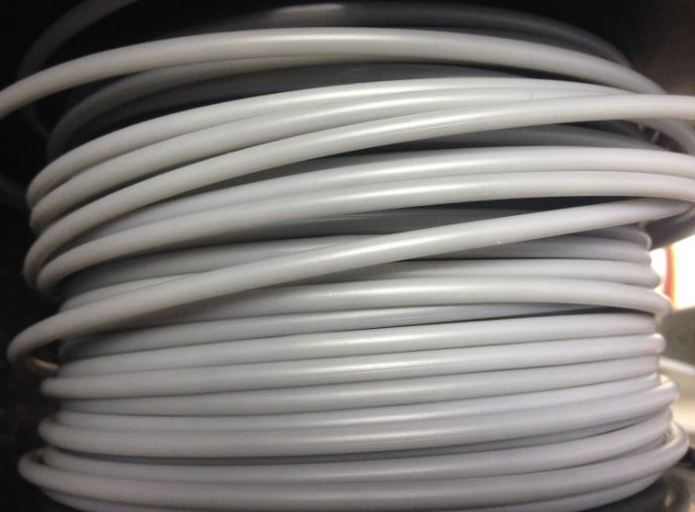
\includegraphics[height=4cm]{Figs4//3_pumice.JPG}
		\end{minipage}
	}
	\subfigure[]{
		\begin{minipage}[t]{0.4\textwidth}
			\centering
			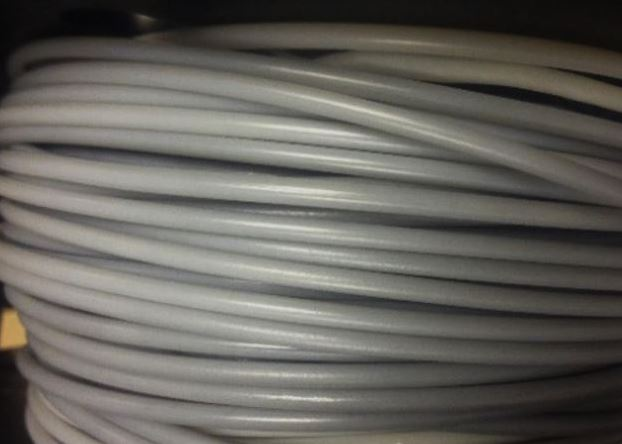
\includegraphics[height=4cm]{Figs4//5_pumice.JPG}
		\end{minipage}
	} 
    \subfigure[]{
		\begin{minipage}[t]{0.4\textwidth}
			\centering
			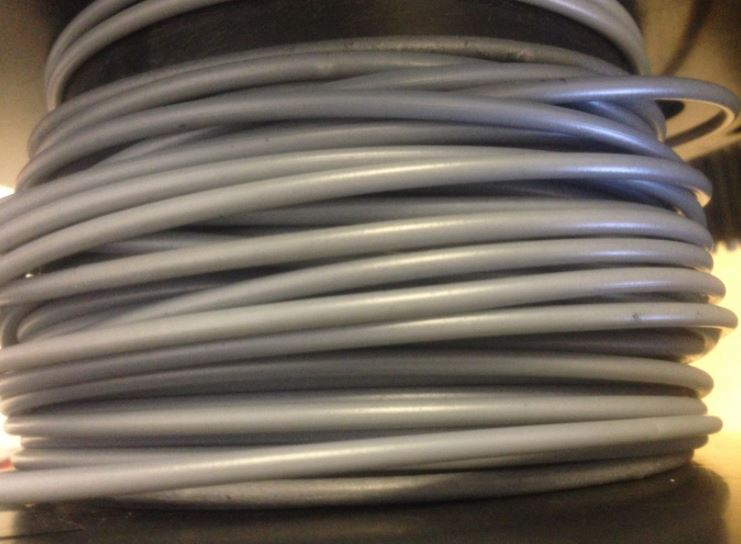
\includegraphics[height=4cm]{Figs4//7_pumice.JPG}
		\end{minipage}
	}
 \subfigure[]{
		\begin{minipage}[t]{0.4\textwidth}
			\centering
			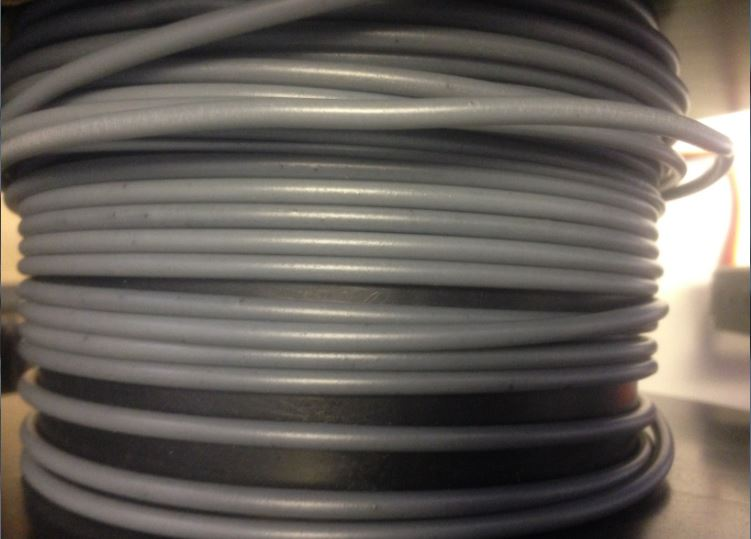
\includegraphics[height=4cm]{Figs4//8_pumice.JPG}
		\end{minipage}
	}
  \caption{The filament samples made of pumice and ABS}{\footnotesize (a)ABS with 3 wt.$\%$ pumice,  (b) ABS with 5 wt.$\%$ pumice, (c) ABS with 7 wt.$\%$ pumice, (d) ABS with 8 wt.$\%$ pumice. }
  \label{Fig:FILAMENTS}
\end{figure}

\section{Analysis}
\subsection{Meaning of adding pumice to filament}
As mentioned in chapter two, this new ink could substitute the traditional material for the space construction. From the data sheet of ABS pellets and pumice, the density of ABS pellets is 1.03 $g/cm^3$ while the density of pumice powder is 2.35 $g/cm^3$. The weight percentage could be easily transformed to voltage percentage as Table \ref{tab:ABS pumice} shows. It is highly certain that the regolith utilisation (In-situ resource utilization ) for 3D printing decreases launch and deep space transit mass and volume requirements. And it seems that this new material production contributes more to the mass saving rather than the volume saving for a space mission.  \\
\begin{table}[htbp]
\centering
\caption{The weight percentage of pumice and corresponding volume percentage}
\begin{tabular}{c  c  c}
\hline
\textbf{Weight percentage} & \textbf{Volume percentage }& \textbf{Density of the blends}\\
\hline
ABS with 0 wt.$\%$ pumice &  ABS with 0.000 vt.$\%$ pumice  &  1.030$g/cm^3$  \\
ABS with 1 wt.$\%$ pumice &  ABS with 0.441 vt.$\%$ pumice  &  1.036$g/cm^3$  \\
ABS with 2 wt.$\%$ pumice &  ABS with 0.887 vt.$\%$ pumice  &  1.041$g/cm^3$  \\
ABS with 3 wt.$\%$ pumice &  ABS with 1.337 vt.$\%$ pumice  &  1.048$g/cm^3$  \\
ABS with 4 wt.$\%$ pumice &  ABS with 1.793 vt.$\%$ pumice  &  1.054$g/cm^3$  \\
ABS with 5 wt.$\%$ pumice &  ABS with 2.255 vt.$\%$ pumice  &  1.060$g/cm^3$  \\
ABS with 6 wt.$\%$ pumice &  ABS with 2.722 vt.$\%$ pumice  &  1.066$g/cm^3$  \\
ABS with 7 wt.$\%$ pumice &  ABS with 3.194 vt.$\%$ pumice  &  1.072$g/cm^3$  \\
ABS with 8 wt.$\%$ pumice &  ABS with 3.671 vt.$\%$ pumice   & 1.078$g/cm^3$ \\
\hline
\end{tabular}
\label{tab:ABS pumice}
\end{table}

\subsection{3D-Printability of pumice filament}
From Table \ref{tab:filament}, it shows the diameter tolerance varies from 0.05mm to 0.10mm since the condition of our equipment was not stable with the same settings. The poor tolerance means that there may be some trouble when we use it in 3D printer.\\
\\
Different problems can be brought by the inhomogeneous filament diameter. A typical case is the extruder failure, a condition where the extrusion fails that no plastic is pushed down to the hot end. This might appear when your filament suddenly shrinks too much for the printer tensioning system and the mechanism offers insufficient pressure to push the filament. The too thin part of the filament will also cause back-flow and over- heating of the material in the hot end since it does not come out with the controlled flow rate. As for the too big filament diameter, there is too much material than the printer supposes it to be in the nozzle head which may block the nozzle head and cause back-flow of the material. Another influence of an increase of filament diameter is that the feeder could grind the surface of the filament and the filament stops moving to the extruder.\\
\\
After all the analysis, the diameter tolerance plays a significant role in its printable ability. Reseaching all extrusion lines in the factory, it’s very hard to go lower 0.05 mm which is already the gold standard. Since our printer was facilitated with an adjustable tensioner and the elastic stepper, it can work well with the filament which has a reasonable diameter tolerance. As we also purchased some filament from industry, we measured the diameter at several places with a calliper. The tolerance of it is 0.10mm which meets the advertised tolerance.\\
\\

\begin{figure}[htbp] % make the image in the middle of paragraph
	\centering
	\subfigure[]{
    \begin{minipage}[t]{1\textwidth}
			\centering
			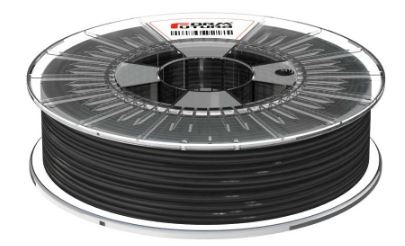
\includegraphics[height=5cm]{Figs4//ABS_easyfil.JPG}
		\end{minipage}
	}
	\subfigure[]{
		\begin{minipage}[t]{1\textwidth}
			\centering
			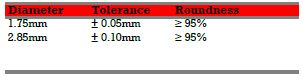
\includegraphics[height=2.5cm]{Figs4//tolerance.JPG}
		\end{minipage}
        }
  \caption{The filament purchased from Formfutura Co.}{\footnotesize  (a)The filament, (b)the diameter tolerance. }
  \label{Fig:filament}
\end{figure}



\chapter{Investigation of 3D Printing Filament}
\renewcommand{\baselinestretch}{\mystretch}
\label{chap:Invest}
%\setlength{\parindent}{0pt}

\section{Methodology}
After the fabrication of the filament, it is essential to investigate its 3D-printability property. Two CAD models were designed to print for different reasons. One was the standard cube and the other one was the waveguide.
\subsection{Cube printing}
Our extrusion of ABS and pumice did not use the same weight of materials that measured before combination since there must be some materials left in the coffee grinder, the hopper and even in a screw. It is not reliable to judge the weight percentage by weighting materials before all procedure. The standard cube may give the information about the density of the printing filament indirectly by weighing it. Then it is possible to deduce the weight percentage of pumice in the new material since the density of ABS and pumice powder are known.\\ 
\begin{figure}[htbp]
  \centering
  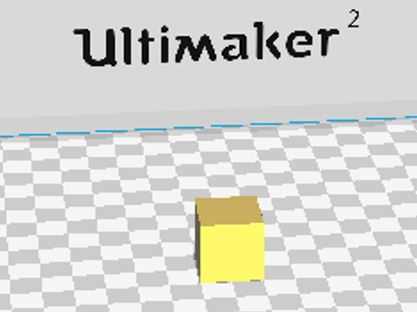
\includegraphics[height=6.5cm,width=10cm]{Figs5//cube_design.JPG}
  \caption[The cube design in Cura]{\footnotesize The cube design in Cura.}
  \label{Fig:cube}
\end{figure}
\subsection{Waveguides printing}
The main task is to print the waveguides with different materials and test their mechanical precision. In particular, it attracted our attention that the roughness of the inner walls of the waveguides which contribute to their performance in practice\cite{d20153}. The waveguides printed with different materials could help us to judge the potential of these materials and find the influences of adding pumice powder to ABS pellets.

\begin{figure}[htbp]
  \centering
  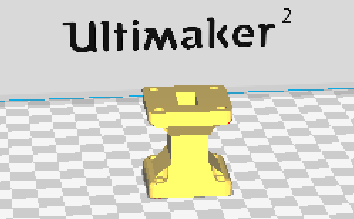
\includegraphics[width=10cm]{Figs//waveguide_design.PNG}
  \caption[The cube design in Cura]{\footnotesize The waveguide design in Cura.}
  \label{Fig:waveguide}
\end{figure}

\section{Experiment}
It is quite frustrated to use pure ABS filament in 3D printer due to the warp of ABS and the difficulties on bed adhesion. There are lots of tips and parameter settings in experiment required to investigate.
\subsection{Design in Cura}
Cura is a multi-functional slicing software that can slice any 3D designs into layers and save the file as G-Code, which could be recognised by the 3D printer. This G-Code file as a text document contains a list of commands for the 3D printer to understand and work with, such as print this part with a speed and print another part with another speed etc. In the Cura software, there are several settings for 3D printing that worth investigating.
\begin{itemize}
\item Printing speed
\end{itemize}
It should be noted that the printing speed has a big influence on the printing quality. In extruding process, the extruding speed is based on the extruding temperature. The print speed should compile with the extruding temperature. The Ultimaker 2 printer has these settings. \\
\\
As for the meaning of speed setting in the Cura software, there is an opportunity to tune the printing speed for different parts of the print. In general, the print speed could be set to 50mm/s and travel speed was 100 mm/s for maximum quality. The initial layer speed should be the lowest one which is 30\% of the print speed for good bed adhesion. The improvements that can be made in Cura are the specific sub-settings of print speed, including infill speed, outer/inner wall speed, top/bottom speed and support speed as Figure\ref{Fig:speed} describes. It is better to slow down the outer wall speed and top/bottom speed as well.
\begin{figure}[htbp]
  \centering
  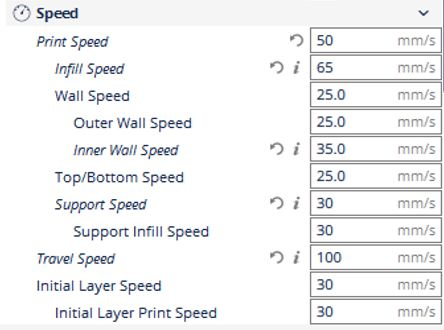
\includegraphics[scale=0.8]{Figs5//speed.JPG}
  \caption[The speed settings in Cura]{\footnotesize The speed settings in Cura.}
  \label{Fig:speed}
\end{figure}

\begin{itemize}
\item Thickness of walls
\end{itemize}
The settings of the shell (i.e. wall thickness and top/bottom thickness) affect the mechanical strength of the printed component. For instance, the 1mm wall thickness makes the waveguides fragile in the middle part while 3mm wall thickness offers the strong body. In general, the sufficient wall thickness setting is 2 or 3 times of the line width. 
\begin{figure}[t] % make the image in the middle of paragraph
	\centering
	\subfigure[]{
    \begin{minipage}[t]{0.4\textwidth}
			\centering
			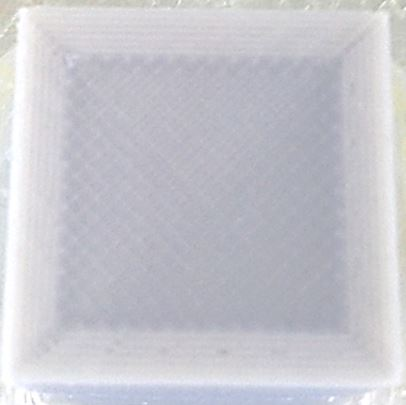
\includegraphics[height=5cm]{Figs5//thickness2.JPG}
		\end{minipage}
	}
	\subfigure[]{
		\begin{minipage}[t]{0.4\textwidth}
			\centering
			
\includegraphics[height=5cm]{Figs5//thickness.jpg}
		\end{minipage}
	} 

  \caption[The setting of wall thickness]{\footnotesize The setting of wall thickness:(a)3mm, (b)3 times of the line width. }
  \label{Fig:thickness}
\end{figure}

\begin{itemize}
\item Infill density
\end{itemize}
Infill is also a significant parameter for 3D printed components. It would cause the warp of ABS if there are lots of solid layers with light infill at the bottom. To be specific, the warp stems from the rapid cooling of the material so that the variety of infill density should be avoided. Since the wall thickness has been decided, the only way to increase the change of infill is using 100$\%$ infill for waveguides printing after several investigations. In Figure\ref{Fig:infill}, it could be shown that the warp of ABS bring the imperfection of the infill part printing while 100$\%$ infill density avoided it. And it needs more material for printing.
\begin{figure}[htbp] % make the image in the middle of paragraph
	\centering
	\subfigure[]{
    \begin{minipage}[t]{0.4\textwidth}
			\centering
			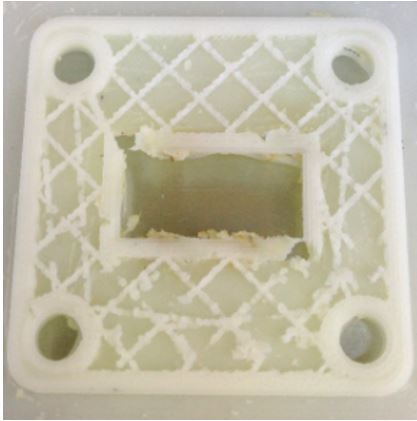
\includegraphics[height=5.5cm]{Figs5//infill1.JPG}
		\end{minipage}
	}
	\subfigure[]{
		\begin{minipage}[t]{0.4\textwidth}
			\centering
			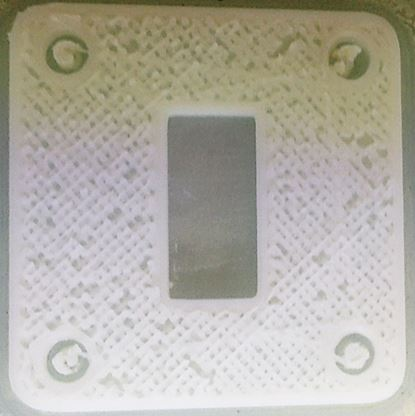
\includegraphics[height=5.5cm]{Figs5//infill2.JPG}
		\end{minipage}
	} 
	\subfigure[]{
		\begin{minipage}[t]{0.4\textwidth}
			\centering
			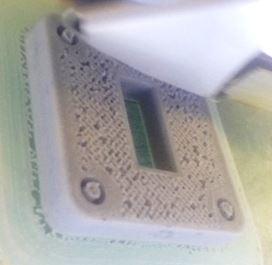
\includegraphics[height=5cm]{Figs5//infill4.JPG}
		\end{minipage}
	} 
	\subfigure[]{
		\begin{minipage}[t]{0.4\textwidth}
			\centering
			\includegraphics[height=5cm]{Figs5//infill5.JPG}
		\end{minipage}
	} 

  \caption[The settings of the infill density]{\footnotesize The settings of the infill density:(a)30$\%$, (b)80$\%$, (c)80$\%$, (d)100$\%$. }
  \label{Fig:infill}
\end{figure}

\begin{itemize}
\item Support structure
\end{itemize}
There are several patterns for support structure in Cura. The best solution depends on your 3D model and the requirements of support part. The support density also should be taken into consideration. Another parameter is Z distance which means the distance from the bottom and top of the support structure to the main printed model. These settings requires delicate designs. As a trade-off, the support structure should be strong but easy to remove. Finally, we have chosen 25$\%$ concentric support structure to print good waveguides. 
\begin{figure}[htbp] % make the image in the middle of paragraph
	\centering
	\subfigure[]{
    \begin{minipage}[t]{0.32\textwidth}
			\centering
			\includegraphics[height=5cm]{Figs5//lines.PNG}
		\end{minipage}
	}
	\subfigure[]{
		\begin{minipage}[t]{0.32\textwidth}
			\centering
			\includegraphics[height=5cm]{Figs5//concentric.PNG}
		\end{minipage}
	} 
 
 \subfigure[]{
		\begin{minipage}[t]{0.31\textwidth}
			\centering
			\includegraphics[height=5cm]{Figs5//geid.PNG}
		\end{minipage}
	} 
     \subfigure[]{
		\begin{minipage}[t]{0.3\textwidth}
			\centering
			\includegraphics[height=5cm]{Figs5//triangles.PNG}
		\end{minipage}
	} 
     \subfigure[]{
		\begin{minipage}[t]{0.3\textwidth}
			\centering
			\includegraphics[height=5cm]{Figs5//zigzag.PNG}
		\end{minipage}
	} 
  \caption[Support patterns]{\footnotesize Support patterns (a)line, (b)concentric, (c)grid, (d)triangles, (e)Zig Zag. }
  \label{Fig:support}
\end{figure}

\begin{itemize}
\item Brim
\end{itemize}
The brim is a nice feature in Cura software to add a single layer flat area around the base of the object, which could decrease the probability of warping. Brim increases the bottom layer area so that it is beneficial to bed adhesion, especially the flatness of the corners.  when printing completes, it could be removed easily. In our experiment, the width of Brim does not make big differences as Figure \ref{Fig:Brim} suggests.
\begin{figure}[htbp] % make the image in the middle of paragraph
	\centering
	\subfigure[]{
    \begin{minipage}[t]{0.45\textwidth}
			\centering
			\includegraphics[height=6cm]{Figs5//10mmbrim.PNG}
		\end{minipage}
	}
	\subfigure[]{
		\begin{minipage}[t]{0.45\textwidth}
			\centering
			\includegraphics[height=6cm]{Figs5//2mmbrim.PNG}
		\end{minipage}
	} 

  \caption[The brim thickness]{\footnotesize The brim thickness of (a)10mm, (b)2mm. }
  \label{Fig:Brim}
\end{figure}

\subsection{Tunable components in UM2}
After finishing the designs in the computer, it is more flexible to adjust some settings in the 3D printer. Some of them should be decided before the printing start while others could be changeable during the printing process\cite{stick}.

\begin{itemize}
\item Bed levelling
\end{itemize}
As the name describes, bed levelling is to make sure that the build plate is completely level. In Ultimaker 2, this work belongs to the maintenance operation. When you level your plate, the distance between nozzle head and the plate is also adjusted.  As the UM2 instructs, a slice of paper was put between the nozzle head and the plate to judge the suitable nozzle distance if you feel a little friction when you remove the paper. In this way, the nozzle distance is about 0.1mm which is exactly the layer thickness. As can be seen in Figure\ref{Fig:bed}, the nozzle distance might be too close for material to come out of the nozzle and adhere evenly or be too far away for material to stick to the bed properly. Therefore, the bed levelling results in the good quality of the first layer.

\begin{figure}[htbp] % make the image in the middle of paragraph
	\centering
	\subfigure[]{
    \begin{minipage}[t]{0.5\textwidth}
			\centering
			\includegraphics[height=6cm]{Figs5//bad_first_layer.JPG}
		\end{minipage}
	}
	\subfigure[]{
		\begin{minipage}[t]{0.45\textwidth}
			\centering
			\includegraphics[height=6cm]{Figs5//bad_adhesion1.JPG}
		\end{minipage}
	} 

  \caption[The distance between nozzle head and build plate]{\footnotesize The distance between nozzle head and build plate is (a)too close, (b)too far.}
  \label{Fig:bed}
\end{figure}

\begin{itemize}
\item Utilization of fans
\end{itemize}
Ultimaker 2 has dual fans for cooling down the extruded material. However, it is mentioned in chapter three that the fans may bring the instability for ABS extrusion. As for bed adhesion, the use of fans has the warping or splitting effect when printing with the ABS filament. Therefore, the fans are not utilised in the experiment. And our 3D printer is placed in a small room other than under the air-conditioner in order to avoid these influences as well.
\begin{figure}[htbp]
  \centering
  \includegraphics[scale=0.4]{Figs5//fan.JPG}
  \caption[The fan installed in UM2]{\footnotesize The fan installed in UM2}
  \label{Fig:fan}
\end{figure}

\begin{itemize}
\item Tension of the feeder
\end{itemize}
There are some effects at the filament feeder that could indicate the extrusion problem. This problem often happens in the hot end, rather than the feeding part. During the experiment, the print fails sometimes since the filament is grinded by the knurled wheel of the feeder. There are two main reasons for this situation. One is that the nozzle head is blocked and the feeder does not give the enough strength to push the material.  The other one is that the filament diameter rapidly changes (shrinks or enlarges) so that the feeder's tension is not suitable for filament moving. Once the filament stops moving, it is easily grinded by the wheel and it never moves again. The solution to this problem is to replace the grinded filament from the Ultimaker 2 by a new piece of filament. It could waste the materials so the good setting at first is very important. The tension of the feeder should be the trade-off to give the enough strength to push the filament as well as not grind the filament.

\begin{figure}[htbp]
  \centering
  \includegraphics[scale=0.6]{Figs5//feeder.JPG}
  \caption[The filament is grinded by the feeder]{\footnotesize The filament is grinded by the feeder.}
  \label{Fig:feeder}
\end{figure}

\begin{itemize}
\item Build platform
\end{itemize}
The glass plate is a good choice for good bed adhesion of materials. As for ABS, it is also advised to heat the build platform to avoid the warping. This method could ensure that the first layer of the ABS does not cool down rapidly, which may result in the shrink of ABS. The recommended temperature of the build platform is from 90$^{\circ}$C to 110$^{\circ}$C.  According to some investigations on it, 105 $^{\circ}$C seems the best setting for our materials. \\
\\
It is also known that a bare glass plate cannot give the strong adhesion. Another tip is to apply a thin layer of glue on it. There are lots of choices of glue. The strongest adhesion will cause the difficulties in removing the products from the build plate while the lightest adhesion cannot meet the requirement. With these considerations, we have used the PVA-based glue stick. The glue is always applied on the cool build plate, It could be dried when heating the plate before printing.  When print was complete, it is easy to remove it after the bed is cooled down to the air temperature entirely and use a wet paper towel with hot water to clean the build platform. 
\begin{itemize}
\item Extruding temperature
\end{itemize}
It is quite tricky for extruding temperature setting. The high temperature could give you the fast extruding speed to some degree while it may bring the back-flow of the material since the ABS is too soft to push. And a lower extruding temperature would slow down the extrusion process. Moreover, the thickness of the layer may be decreased and there may be some gaps between each line. It means that the extruding speed cannot follow the print speed. The latter case could be dealt with by slow down the print speed. For safety, we set 240 $^{\circ}$C as the extruding temperature in the 3D printer. 
\begin{itemize}
\item Printing speed
\end{itemize}
In Ultimaker 2, the print speed could be tuned anytime during printing. The speed is controlled by the percentage of designed speed in Cura. For example, setting 50 mm/s print speed in Cura and 30$\%$ speed in UM2 offers 15mm/s as the true speed. It is an advantage of the printer that we can manually change the speed according to the performance rather than discard the print and start a new one.
\begin{figure}[htbp] % make the image in the middle of paragraph
	\centering
	\subfigure[]{
    \begin{minipage}[t]{0.45\textwidth}
			\centering
			\includegraphics[height=6cm]{Figs5//speed1.JPG}
		\end{minipage}
	}
	\subfigure[]{
		\begin{minipage}[t]{0.45\textwidth}
			\centering
			\includegraphics[height=6cm]{Figs5//speed2.JPG}
		\end{minipage}
        }
  \caption[The filament made with different speed]{\footnotesize The filament made with (a)70$\%$ speed, (b)50$\%$ speed. }
  \label{Fig:speed}
\end{figure}
\subsection{3D printing results}
The basic judgment of the success of the print is the first layer. If the first layer is sufficiently nice, we could continue to print all model otherwise we should change the settings and start a new one again. Figure \ref{Fig:first layer} offers the examples of first layers. And all of our produced filament could print a successful first layer in UM2.
\begin{figure}[htbp]
  \centering
  \includegraphics[scale=0.65]{Figs5//first_layer.JPG}
  \caption[The different situations of the first layer]{\footnotesize The different situations of the first layer.}
  \label{Fig:first layer}
\end{figure}
\begin{itemize}
\item Cubes
\end{itemize}
The infill setting of the cube is 100$\%$ due to its design aim that is to measure the density of the material. At first, we only print a 1 $cm^3/g$ to test the density of the filament. However, the result shows a big measure error and the printed cube is very irregular as Figure\ref{Fig:bad cube} represents. The volume of it is too small and the print settings including print speed wall thickness are not proper. In this case, an 8 $cm^3/g$ cube is more reasonable.
\begin{figure}[t]
  \centering
  \includegraphics[scale=0.6]{Figs5//bad_cube.JPG}
  \caption[The 3D-printed 1 $cm^3/g$ cube]{\footnotesize The 3D-printed 1 $cm^3/g$ cube.}
  \label{Fig:bad cube}
\end{figure}
Since it is composed of lots of solid layers, the corners of it warp easily due to the different cooling speed of ABS at the corners. And there are air bubbles in the filament which result in the thinner layer than the printer suppose it to be. Therefore, the final results are still not good as shown in Figure \ref{Fig:cubes}. The weight of each cube is described in Table \ref{tab:cube density}. The density calculated by this measurement is really different from the theoretical one.
\begin{table}[htbp]
\centering
\caption {The weight and density of the printed cubes}
\begin{tabular}{c c c c}
\hline
\textbf{Weight} & \textbf{Material} & \textbf{Measured density} & \textbf{theoretical density}\\
\hline
7.00g & ABS with 0 wt.$\%$ pumice &  0.875 $g/cm^3$ &  1.030$g/cm^3$ \\
7.11g & ABS with 1 wt.$\%$ pumice & 0.889 $g/cm^3$ &  1.036$g/cm^3$  \\
6.48g & ABS with 2 wt.$\%$ pumice &  0.81 $g/cm^3$&  1.041$g/cm^3$  \\
6.86g & ABS with 3 wt.$\%$ pumice &  0.858 $g/cm^3$&  1.048$g/cm^3$  \\
6.45g & ABS with 4 wt.$\%$ pumice &  0.806 $g/cm^3$&  1.054$g/cm^3$  \\
6.94g & ABS with 5 wt.$\%$ pumice &  0.868 $g/cm^3$&  1.060$g/cm^3$  \\
6.60g & ABS with 6 wt.$\%$ pumice &  0.825 $g/cm^3$&  1.066$g/cm^3$  \\
\hline
\end{tabular}
\label{tab:cube density}
\end{table}

\begin{figure}[htbp] % make the image in the middle of paragraph
	\centering
	\subfigure[]{
    \begin{minipage}[t]{0.35\textwidth}
			\centering
			\includegraphics[height=4.6cm,width=4.6cm]{Figs5//0.JPG}
		\end{minipage}
	}
	\subfigure[]{
		\begin{minipage}[t]{0.35\textwidth}
			\centering
			\includegraphics[height=4.6cm,width=4.6cm]{Figs5//1.JPG}
		\end{minipage}
        }
        \subfigure[]{
    \begin{minipage}[t]{0.35\textwidth}
			\centering
			\includegraphics[height=4.6cm,width=4.6cm]{Figs5//2.JPG}
		\end{minipage}
	}
        \subfigure[]{
    \begin{minipage}[t]{0.35\textwidth}
			\centering
			\includegraphics[height=4.6cm,width=4.6cm]{Figs5//3.JPG}
		\end{minipage}
	}
    \subfigure[]{
    \begin{minipage}[t]{0.35\textwidth}
			\centering
			\includegraphics[height=4.6cm]{Figs5//4.JPG}
		\end{minipage}
	}
    \subfigure[]{
    \begin{minipage}[t]{0.35\textwidth}
			\centering
			\includegraphics[height=4.6cm,width=4.6cm]{Figs5//5.jpg}
		\end{minipage}
	}
    \subfigure[]{
    \begin{minipage}[t]{0.35\textwidth}
			\centering
			\includegraphics[height=4.6cm]{Figs5//6.JPG}
		\end{minipage}
	}
 
  \caption[The 3D-printed cubes]{\footnotesize The 3D-printed cubes made of(a)no pumice, (b)1 wt.$\%$ pumice, (c)2 wt.$\%$ pumice, (d)3 wt.$\%$ pumice, (e)4 wt.$\%$ pumice, (f)5 wt.$\%$ pumice, (g)6 wt.$\%$ pumice. }
  \label{Fig:cubes}
\end{figure}
\begin{figure}[htbp] % make the image in the middle of paragraph
	\centering
	\subfigure[]{
    \begin{minipage}[t]{0.2\textwidth}
			\centering
			\includegraphics[height=2.5cm]{Figs5//block0.jpg}
		\end{minipage}
	}
    \subfigure[]{
    \begin{minipage}[t]{0.2\textwidth}
			\centering
			\includegraphics[height=2.5cm]{Figs5//block1.jpg}
		\end{minipage}
	}
    \subfigure[]{
    \begin{minipage}[t]{0.2\textwidth}
			\centering
			\includegraphics[height=2.5cm]{Figs5//block2.jpg}
		\end{minipage}
	}
    \subfigure[]{
    \begin{minipage}[t]{0.2\textwidth}
			\centering
			\includegraphics[height=2.5cm]{Figs5//block3.jpg}
		\end{minipage}
	}
  \subfigure[]{
    \begin{minipage}[t]{0.2\textwidth}
			\centering
			\includegraphics[height=2.5cm]{Figs5//block4.jpg}
		\end{minipage}
	}
     \subfigure[]{
    \begin{minipage}[t]{0.2\textwidth}
			\centering
			\includegraphics[height=2.5cm]{Figs5//block5.jpg}
		\end{minipage}
	}
     \subfigure[]{
    \begin{minipage}[t]{0.2\textwidth}
			\centering
			\includegraphics[height=2.5cm]{Figs5//block6.jpg}
		\end{minipage}
	}
  \caption[The infill lines on the cubes]{\footnotesize The infill lines on the cubes made with (a)no pumice, (b)1 wt.$\%$ pumice, (c)2 wt.$\%$ pumice, (d)3 wt.$\%$ pumice, (e)4 wt.$\%$ pumice, (f)5 wt.$\%$ pumice, (g)6 wt.$\%$ pumice.}
  \label{Fig:cube layer}
\end{figure}
\begin{figure}[htbp] % make the image in the middle of paragraph
	\centering
	\subfigure[]{
    \begin{minipage}[t]{0.2\textwidth}
			\centering
			\includegraphics[height=2.5cm]{Figs5//cblock0.jpg}
		\end{minipage}
	}
    \subfigure[]{
    \begin{minipage}[t]{0.2\textwidth}
			\centering
			\includegraphics[height=2.5cm]{Figs5//cblock1.jpg}
		\end{minipage}
	}
    \subfigure[]{
    \begin{minipage}[t]{0.2\textwidth}
			\centering
			\includegraphics[height=2.5cm]{Figs5//cblock2.jpg}
		\end{minipage}
	}
    \subfigure[]{
    \begin{minipage}[t]{0.2\textwidth}
			\centering
			\includegraphics[height=2.5cm]{Figs5//cblock3.jpg}
		\end{minipage}
	}
  \subfigure[]{
    \begin{minipage}[t]{0.2\textwidth}
			\centering
			\includegraphics[height=2.5cm]{Figs5//cblock4.jpg}
		\end{minipage}
	}
     \subfigure[]{
    \begin{minipage}[t]{0.2\textwidth}
			\centering
			\includegraphics[height=2.5cm]{Figs5//cblock5.jpg}
		\end{minipage}
	}
     \subfigure[]{
    \begin{minipage}[t]{0.2\textwidth}
			\centering
			\includegraphics[height=2.5cm]{Figs5//cblock6.jpg}
		\end{minipage}
	}
  \caption[The wall lines on the cubes]{\footnotesize The wall lines on the cubes made of (a)no pumice, (b)1 wt.$\%$ pumice, (c)2 wt.$\%$ pumice, (d)3 wt.$\%$ pumice, (e)4 wt.$\%$ pumice, (f)5 wt.$\%$ pumice, (g)6 wt.$\%$ pumice. }
  \label{Fig:cube layer2}
\end{figure}
As Figure \ref{Fig:cube layer} and \ref{Fig:cube layer2} shows, the details of the cubes are different which are captured by the microscope and connected camera. The one made by pure ABS has almost no gaps between lines but it warps seriously. Considering the geometrical accuracy and the gaps between lays and lines, the best one is made by 5 wt.\% pumice. Checking their corresponding filament, the big gaps between lines are stem from the diameter which is larger than 3.00mm or smaller than 2.80mm. The UM2 is quite sensitive to the size of the filament. And the pumice powder decreases the level of warp according to the geometrical accuracy of the cubes. 

\begin{itemize}
\item Waveguides
\end{itemize}
The printing of waveguides is the most time-consuming work in this project. The challenge is derived from the materials we utilised are really new. The printability of them is uncertain. The most printable filament is fabricated with 2 wt.$\%$ pumice and ABS and has 2.85-3.05mm diameter. It cannot be denied that filament consistency also influenced the printability of it but the guess work could demonstrate whether it is printable. As for the practical usage of the waveguides, the flatness of inner wall contributes a lot. Therefore, it is essential to compare the performance of their inner wall. 

\begin{figure}[htbp] % make the image in the middle of paragraph
	\centering
	\subfigure[]{
    \begin{minipage}[t]{0.35\textwidth}
			\centering
			\includegraphics[height=5cm]{Figs5//0_pumice.JPG}
		\end{minipage}
	}
	\subfigure[]{
		\begin{minipage}[t]{0.35\textwidth}
			\centering
			\includegraphics[height=5cm]{Figs5//1_pumice.JPG}
		\end{minipage}
        }
        \subfigure[]{
    \begin{minipage}[t]{0.35\textwidth}
			\centering
			\includegraphics[height=5cm]{Figs5//2_pumice.JPG}
		\end{minipage}
	}
        \subfigure[]{
    \begin{minipage}[t]{0.35\textwidth}
			\centering
			\includegraphics[height=5cm]{Figs5//3_pumice.JPG}
		\end{minipage}
	}
    \subfigure[]{
    \begin{minipage}[t]{0.35\textwidth}
			\centering
			\includegraphics[height=5cm]{Figs5//4_pumice.JPG}
		\end{minipage}
	}
    \subfigure[]{
    \begin{minipage}[t]{0.35\textwidth}
			\centering
			\includegraphics[height=5cm]{Figs5//5_pumice.JPG}
		\end{minipage}
	}
    \subfigure[]{
    \begin{minipage}[t]{0.35\textwidth}
			\centering
			\includegraphics[height=5cm]{Figs5//6_pumice.JPG}
		\end{minipage}
	}
    \subfigure[]{
    \begin{minipage}[t]{0.35\textwidth}
			\centering
			\includegraphics[height=5cm]{Figs5//7_pumice.JPG}
		\end{minipage}
	}
  \caption[The 3D-printed waveguides]{\footnotesize The 3D-printed waveguides made of (a)no pumice, (b)1 wt.$\%$ pumice, (c)2 wt.$\%$ pumice, (d)3 wt.$\%$ pumice, (e)4 wt.$\%$ pumice, (f)5 wt.$\%$ pumice, (g)6 wt.$\%$ pumice, (h)7 wt.$\%$ pumice.}
  \label{Fig:waveguides}
\end{figure}

\section{Analysis}
\subsection{The distribution of the pumice powder in filament}

According to the bad performance of the filament containing 7 wt.\% pumice, the main reason is the air bubbles in the filament and its brittleness. The pumice powder could be seen with the microscope in Figure \ref{Fig:pumice}. Compared with the corresponding calibration, the size of pumice powder is between 2-12$\mu$m. From the microscope pictures of the filament, it is easy to find the small pumice particles. It is obvious that there is an air bubble in Figure\ref{Fig:slice} (b) with lots of pumice particles nearby. Based on these pictures, the distribution of the pumice powder in the filament is not uniform and the most of the powder is around the air bubbles. It could be deduced that the air bubble and the converge of pumice particles could make the filament very brittle and even block the nozzle head during printing.\\
\\
There is a high possibility that the air bubbles could be avoided in a very dry environment. It is necessary to use an oven to slightly melt ABS pellets and dry pumice powder rather than the coffee grinder. In order to distribute pumice powder evenly in the filament, the screw in extruder should be longer and multi-functional to mix the ABS and pumice sufficiently.
\begin{figure}[htbp] % make the image in the middle of paragraph
	\centering
    \subfigure[]{
    \begin{minipage}[t]{0.45\textwidth}
			\centering
			\includegraphics[height=5cm]{Figs5//pumi.jpg}
		\end{minipage}
	}
    \subfigure[]{
    \begin{minipage}[t]{0.45\textwidth}
			\centering
			\includegraphics[height=5cm]{Figs5//calibration.jpg}
		\end{minipage}
	}
  \caption{The microtexture of the pumice powder}{\footnotesize (a)pumice powder (b)corresponding calibration }
    \label{Fig:pumice}
\end{figure}

\begin{figure}[htbp] % make the image in the middle of paragraph
	\centering
    \subfigure[]{
    \begin{minipage}[t]{0.45\textwidth}
			\centering
			\includegraphics[height=5cm]{Figs5//ABS.jpg}
		\end{minipage}
	}
    \subfigure[]{
    \begin{minipage}[t]{0.45\textwidth}
			\centering
			\includegraphics[height=5cm]{Figs5//ABS7p.jpg}
		\end{minipage}
	}
  \caption[The microtexture of the filament]{\footnotesize The microtexture of the filament made by (a)pure ABS, (b)7 wt.$\%$ pumice and ABS. }
  \label{Fig:slice}
\end{figure}

\subsection{The measurement error of cubes}
From Table \ref{tab:cube density}, it is obvious that the measurement error is quite big. Therefore, the density calculated by this method is not reliable. The main reason behind it is the bad quality of the printed cubes. The geometrical accuracy of the cubes is quite high due to the warp of ABS. And the extruded filament is thinner than the printer supposes it to be so that there are some gaps between the layers. The cubes are not 100$\%$ filled inside which make the weight is lighter than the theoretical one. The effect of pumice powder is not only the brittleness actually. The filament made by pumice powder and ABS contains air inside and it is easier to absorb moisture from the environment than the pure ABS filament. And the average diameter of the filament is smaller than 2.85mm as the printer's default setting. In this case, the real volume of the printed material is less than our design of the model when the printer extrudes the specific length of the filament as the G-code commands. The more pumice powder in the filament, the worse quality of the prints. As for the density of the manufactured filament, the printability of the filament is sacrificed for the lighter weight of the filament since it contains air bubbles, which is not meaningful.

\subsection{The geometrical accuracy of waveguides}
The overall results indicate the pumice powder could improve the quality of prints when its weight percentage is lower than 6$\%$ according to the equipment facilitated in this project. Otherwise, it cannot be printable when the weight percentage of pumice powder is beyond 7\%. Focused on the inner wall flatness of the waveguides, the worst one is produced by 7 wt.$\%$ pumice. It is because the filament is too brittle to print with and the nozzle is easily blocked during the printing.

\begin{figure}[htbp] % make the image in the middle of paragraph
	\centering
	\subfigure[]{
    \begin{minipage}[t]{0.35\textwidth}
			\centering
			\includegraphics[height=5cm]{Figs5//in0.JPG}
		\end{minipage}
	}
	\subfigure[]{
		\begin{minipage}[t]{0.35\textwidth}
			\centering
			\includegraphics[height=5cm]{Figs5//in1.JPG}
		\end{minipage}
        }
        \subfigure[]{
    \begin{minipage}[t]{0.35\textwidth}
			\centering
			\includegraphics[height=5cm]{Figs5//in2.JPG}
		\end{minipage}
	}
        \subfigure[]{
    \begin{minipage}[t]{0.35\textwidth}
			\centering
			\includegraphics[height=5cm]{Figs5//in3.JPG}
		\end{minipage}
	}
    \subfigure[]{
    \begin{minipage}[t]{0.35\textwidth}
			\centering
			\includegraphics[height=5cm]{Figs5//in4.JPG}
		\end{minipage}
	}
     \subfigure[]{
    \begin{minipage}[t]{0.35\textwidth}
			\centering
			\includegraphics[height=5cm]{Figs5//in5.JPG}
		\end{minipage}
	}
    \subfigure[]{
    \begin{minipage}[t]{0.35\textwidth}
			\centering
			\includegraphics[height=5cm]{Figs5//in6.JPG}
		\end{minipage}
	}
    \subfigure[]{
    \begin{minipage}[t]{0.35\textwidth}
			\centering
			\includegraphics[height=5cm]{Figs5//in7.JPG}
		\end{minipage}
	}
  \caption[The inner wall of the waveguides]{\footnotesize The inner wall of the waveguides made by (a)no pumice, (b)1 wt.$\%$ pumice, (c)2 wt.$\%$ pumice, (d)3 wt.$\%$ pumice, (e)4 wt.$\%$ pumice, (f)5 wt.$\%$ pumice, (g)6 wt.$\%$ pumice, (h)7 wt.$\%$ pumice.}
  \label{Fig:inner}
\end{figure}



\chapter{Conclusion}
\renewcommand{\baselinestretch}{\mystretch}
\label{chap:Conclu}
%\setlength{\parindent}{0pt}

\section{Contribution to 3D printing in space}
In this project, the main work is applying lunar and martian dust simulants for the entire FDM technique, including the manufacture of the printable filament and the 3D printing of microscope components. The key challenges are the combination of ABS pellets, pumice powder and the investigation of the filament printability. The solution to the first problem is slightly melting the ABS pellets so the very fine pumice powder can uniform lyattached to their surface. Then the sufficient mixture is processed by the screw of the extruder. The finding of the latter one is that the filament made of 1 wt.\%- 7 wt.\% could be printable in UM2 with the settings of 240$^{\circ}$C extruding temperature without fans, 105$^{\circ}$C build plate with PVA based glue and a relatively low print speed. In particular, a small quantity of pumice powder could improve the printability of ABS based filament. This finding offers the potential that Lunar and Mars dust could be applied as a raw material for FDM technique. 

\section{Limitations of this project}
The findings of this study are restricted to the unprofessional equipments. The printability of the filament could be better if the extruder works better. The lack of the mechanical test of the 3D-printed waveguides means that we cannot recognize the influence of the pumice powder on the prints and the value of the 3D-printed waveguides clearly. \\
\\
There is no accurate data representing how much pumice contained in the filament. Therefore, our experiment is a guess work that demonstrates the possibility of using Lunar/Mars Dust simulants in the FDM system.

\section{Future work}

\subsection{The utilisation of Topas polymers as the base material}
This study has addressed only the combination of ABS pellets and Lunar/Mars dust simulants. There is another interesting material called Topas polymers (8007S-04, TOPAS Advanced Polymer Co.). This material has a tricky property that it is softer than ABS at its glass transition temperature (i.e. 78$^{\circ}$C). Due to this mechanical property, the extruder Noztek Pro seems not very suitable for Topas filament manufacturing as the diameter could have a quite big tolerance. The extruded Topas filament by Noetek Pro extruder could be seen in Figure \ref{Fig:Topaz polymer} below. Its diameter is not uniform, which varies from 2.35mm to 2.78mm with 180$^{\circ}$C extruding temperature specifically. The Topas filament stretches a lot when it goes through the filament guiding gate of the extruder. It is highly certain that this kind of polymers could produce a printable filament with other extruder or equipment. \\
\\
The outstanding property of it is the transparent colour which is an ideal material to produce the optical components. And there is a strong possibility of the combination of Topas and Lunar/Mars dust since Topas polymers are sticky at high temperature while the latter increases the brittleness of the filament.  
\begin{figure}[htbp]
  \centering
  \includegraphics[scale=0.5]{Figs5//topaz_filament.JPG}
  \caption[The Topas filament]{\footnotesize The Topas filament.}
  \label{Fig:Topaz polymer}
\end{figure}

\subsection{The restriction of using ABS with Lunar and Mars regolith}
It seems the blends of ABS and Lunar/Mars regolith have some limitations for FDM technique. The brittleness of the filament made of the blends could cause the failure of printing. There is a strong possibility to add some material to make it soft and sticky at extruding temperature or use other thermoplastics to mix with the blends of ABS and Lunar/Mars dust simulants. This material might decrease the brittleness of the mixture so that the proportion of Lunar/Mars dust could be increased.


%%%%%%%%%%%%%%%%%%%%%%
% The reference list.%
%%%%%%%%%%%%%%%%%%%%%%

\renewcommand{\baselinestretch}{1}

% Note: put the bib style and bib file you use here.
\bibliographystyle{IEEEtran}
\bibliography{IEEEabrv,references}

%%%%%%%%%%%%%%%%%%%%%%%%%%%%%
% The end of reference list.%
%%%%%%%%%%%%%%%%%%%%%%%%%%%%% 
\fancyhead[RE]{\emph{References}}

\appendix
\renewcommand{\baselinestretch}{2}
\chapter{ABS Pellets Data Sheet}
\label{App:ABS}
\newpage
\centering
\includegraphics[page=1,scale=0.71]{ABS_Datasheet.pdf}
\includegraphics[page=2,scale=0.71]{ABS_Datasheet.pdf}
\includegraphics[page=3,scale=0.71]{ABS_Datasheet.pdf}
\chapter{Pumice Powder Data Sheet}
\label{App:pumice}
\newpage
\centering
\includegraphics[page=1,scale=0.75]{powdered_pumice_very_fine_datasheet.pdf}
\includegraphics[page=2,scale=0.75]{powdered_pumice_very_fine_datasheet.pdf}
\includegraphics[page=3,scale=0.75]{powdered_pumice_very_fine_datasheet.pdf}
\includegraphics[page=4,scale=0.75]{powdered_pumice_very_fine_datasheet.pdf}
\includegraphics[page=5,scale=0.75]{powdered_pumice_very_fine_datasheet.pdf}
\includegraphics[page=6,scale=0.75]{powdered_pumice_very_fine_datasheet.pdf}
\includegraphics[page=7,scale=0.75]{powdered_pumice_very_fine_datasheet.pdf}
\includegraphics[page=8,scale=0.75]{powdered_pumice_very_fine_datasheet.pdf}
\includegraphics[page=9,scale=0.75]{powdered_pumice_very_fine_datasheet.pdf}
\chapter{Topas Polymer Data Sheet}
\label{App:topaz}
\newpage
\centering
\includegraphics[page=1,scale=0.75]{Topas.pdf}
\appendix


\fancyhead[RE]{\emph{Appendix}}
%%%%%%%%%%%%%%%%%%%%%%%%%%%%%%
% The end of a LaTeX document
\end{document}

%%%%%%%%%%The END%%%%%%%%%%%%%%%%%%%% 